\subsection{The Hahn-Banach theorem (analytic form)}

THEOREM 1 (Hahn-Banach). --- Let p be a sub-linear function on a vector space E. Let V be a vector subspace of E and f a linear form on V such that, for all \(y \in V\) , we have \(f(y) \leqslant p(y)\) . Then there exists a linear form h on E that is an extension of f and such that \(h(x) \leqslant p(x)\) for \(x \in E\) .

The set of pairs \((x, a)\) such that \(p(x) \leqslant a\) is a convex subset P of the vector space \(E_{1} = E \times R\) (II, p.~17, prop. 19), and it is clearly a pointed cone. Let \(V_{1}\) be the subspace \(V \times R\) of \(E_{1}\) and \(g(y, a) = -f(y) + a\) for each point \((y, a) \in V_{1}\) . Then g is a positive linear form for the preorder structure on \(V_{1}\) defined by \(P \cap V_{1}\) ; for if \((y, a) \in P \cap V_{1}\) , then \(a \geqslant p(y) \geqslant f(y)\) , therefore \(g(y, a) \geqslant 0\) . Next let \((x, a) \in E_{1}\) ; we show that \((x, a)\) is less than a point of \(V_{1}\) for the preorder defined by P. If \((x', a') \in V_{1}\) then \((x, a) \leqslant (x', a')\) if, and only if, \(p(x' - x) \leqslant a' - a\) , taking \(a' \geqslant p(-x) + a\) , we see that \((0, a')\) of \(V_{1}\) satisfies the requirements. Thus we can apply prop. 1 of II, p.~21; there is a linear form u on \(E_{1}\) extending g and positive for the preorder defined by P. Therefore \(u(0, 1) = g(0, 1) = 1\) and u is of the form \(u(x, a) = -h(x) + a\) , where h is a linear form on E that extends f; further, for all \(x \in E\) and all \(a \geqslant p(x)\) , we have \(h(x) \leqslant a\) , therefore \(h(x) \leqslant p(x)\) . Q.E.D.

COROLLARY 1. --- Let p be a semi-norm on the vector space E. Let V be a vector subspace of E and f a linear form on V such that \(|f(y)| \leqslant p(y)\) for all \(y \in V\) . Then there exists a linear form h defined on E which is an extension of f and is such that \(|h(x)| \leqslant p(x)\) for \(x \in E\) .

For a semi-norm \(q\) and a linear form \(g\) on \(\mathbf{E}\) , the relation \(g \leqslant q\) is the same as \(|g| \leqslant q\) . The corollary follows from th. 1.

COROLLARY 2. --- Let p be a semi-norm on the vector space E. Given a point \(x_{0} \in E\) , there exists a linear form f defined over E, such that \(f(x_{0}) = p(x_{0})\) and that \(|f(x)| \leqslant p(x)\) for all \(x \in E\) .

Apply cor. 1 to the vector subspace, V, generated by \(x_0\) and to the linear form \(\xi x_0 \mapsto \xi p(x_0)\) defined over V.

COROLLARY 3. --- Let V be a vector subspace of the normed space E and let f be a continuous linear form over V; then there exists a continuous linear form h defined over E which extends f and is of the same norm (GT, X, § 3.2).

Apply cor. 1, taking \(p(x) = \| f \| \cdot \| x \|\) , which gives \(\| h \| \leqslant \| f \|\) ; but clearly \(\| h \| \geqslant \| f \|\) , and the corollary follows.

The conclusion of cor. 3 is not necessarily valid for continuous linear mappings of a normed space into an arbitrary normed space (IV, p.~55, exerc. 16, c) and V, p.~65, exerc. 22).

\section{LOCALLY CONVEX SPACES}

\subsection{Definition of a locally convex space}

DEFINITION 1. --- A topological vector space is locally convex (real) if there exists a fundamental system of neighbourhoods of 0 that are convex sets.

Such a space is called a locally convex space. Its topology is called a locally convex topology.

The topological vector spaces over \(\mathbf{R}\) which we study in the rest of this book are nearly all locally convex.

If V is a convex neighbourhood of 0 in the locally convex space E, then \(V \cap (-V)\) is a symmetric convex neighbourhood of 0. As the closure of a convex set is convex (II, p.~13, prop. 14) it follows from I, p.~7, prop. 4 that the neighbourhoods of 0 in E which are closed, symmetric and convex, form a fundamental system of neighbourhoods invariant under homotheties of centre 0 and ratio \(\neq 0\) .

PROPOSITION 1. --- Let S be a filter base on a vector space E formed from sets that are absorbent, symmetric and convex. Then the set V of transforms of the sets of S by homotheties of ratio \textgreater{} 0 is a fundamental system of neighbourhoods of 0 for a locally convex topology on E.

Clearly \(\mathfrak{B}\) is a filter base satisfying \((\mathrm{EV}_{\mathrm{I}})\) and \((\mathrm{EV}_{\mathrm{II}})\) of I, p.~7, prop. 4; it also satisfies \((\mathrm{EV}_{\mathrm{III}})\) since if \(\mathbf{V} \in \mathfrak{S}\) then \(\frac{1}{2}\mathbf{V} + \frac{1}{2}\mathbf{V} = \mathbf{V}\) .

Note that if \(\mathcal{T}\) is the locally convex topology on E having \(\mathfrak{V}\) for a fundamental system of neighbourhoods of 0, then the sets \((1/n)\) V, where \(n\) varies in the integers \(>0\) and V varies in \(\mathfrak{S}\) , form a fundamental system of neighbourhoods of 0 for the topology \(\mathcal{T}\) . Then \(\mathcal{T}\) is Hausdorff, if and only if, for every \(x \neq 0\) in E there exists an integer \(n\) and a set \(\mathrm{V} \in \mathfrak{S}\) , such that \(nx \notin \mathrm{V}\) ; if, further, \(\mathfrak{S}\) is enumerable, then the topology \(\mathcal{T}\) is a metrisable locally convex topology. Conversely, it is clear that if \(\mathcal{T}\) is a metrisable locally convex topology, then there exists an enumerable fundamental system of closed symmetric convex neighbourhoods of 0 for \(\mathcal{T}\) .

COROLLARY. --- The topology \(\mathcal{T}\) of a topological vector space E, is defined by a set of semi-norms (II, p.~3) if, and only if, \(\mathcal{T}\) is locally convex.

The condition is necessary since every semi-norm on E is a convex function, and so, for \(\alpha > 0\) , the set of \(x \in E\) for which \(p(x) \leqslant \alpha\) , is convex (II, p.~17, corollary). Conversely if V is a symmetric, closed, convex neighbourhood of 0 in E, the gauge p of V is a semi-norm on E such that V is the set of points x of E satisfying \(p(x) \leqslant 1\) (II, p.~20, prop. 23).

This shows further that a locally convex topology \(\mathcal{T}\) is defined by the set of all semi-norms that are continuous for \(\mathcal{T}\) . Further, if \(\mathcal{T}\) is metrisable, then it is defined by an enumerable set of semi-norms.

From the corollary to prop. 1, all the results of § 1 on topologies defined by sets of semi-norms apply in particular to locally convex topologies over real vector spaces. A locally convex Hausdorff space E has a completion \(\hat{E}\) that is locally convex. A complete, metrisable locally convex space is called a Fréchet space; every Banach space is a Fréchet space.

PROPOSITION 2. --- Let f be a continuous linear form defined over a vector subspace M, of a locally convex space E; then there exists a continuous linear form h that is defined over E and is an extension of f.

From the corollary above and II, p.~7, cor. 2, there exists a continuous semi-norm \(p\) on \(\mathbf{E}\) , such that \(|f(y)| \leqslant p(y)\) for all \(y \in \mathbf{M}\) . By the Hahn-Banach th. (II, p.~23, cor. 1) there exists a linear form \(h\) on \(\mathbf{E}\) that extends \(f\) and is such that \(|h(x)| \leqslant p(x)\) for all \(x \in \mathbf{E}\) , and this implies that \(h\) is continuous (II, p.~6, prop. 5).

Remark. --- If g is a continuous linear mapping of M in the product space \(R^{I}\) , then there exists a continuous linear mapping h of E in \(R^{I}\) that is an extension of g; for writing \(g = (g_{\mathrm{t}})\) , where the \(g_{t}\) are continuous linear forms defined over M, there is an extension \(h_{t}\) of \(g_{t}\) for each \(t \in I\) , such that \(h_{t}\) is a continuous linear form over E. The continuous linear mapping \(h = (h_{\mathrm{t}})\) has the required properties.

Note that if \(\mathbf{F}\) is a locally convex Hausdorff space and \(g\) a continuous linear mapping of \(\mathbf{M}\) in \(\mathbf{F}\) , then there does not necessarily exist a continuous linear mapping of \(\mathbf{E}\) in \(\mathbf{F}\) which is an extension of \(g(\mathrm{IV},\mathrm{p.~55},\mathrm{exerc.~16},c))\) . However there does exist such an extension when \(\mathbf{M}\) is finite dimensional (cf.~cor. 2, below).

COROLLARY 1. --- Let E be a locally convex space. If \(x_0 \in E\) is not in the closure of \(\{0\}\) , then there exists a continuous linear form \(f\) defined over E with \(f(x_0) \neq 0\) .

Apply prop. 2 to the one dimensional vector space M generated by \(x_0\) and to the linear form \(\xi x_0 \mapsto \xi\) defined over M, which, by I, p.~12, prop. 2, is continuous.

COROLLARY 2. --- Let M be a finite dimensional vector subspace of E, a locally convex Hausdorff space. Then there exists a closed vector subspace N of E, which is the topological complement of M in E.

There exists a topological complement to M in E if, and only if, the identity mapping of M on itself can be extended to a continuous linear mapping of E on M, which mapping is then necessarily a continuous projector (GT, III, § 6.2, corollary). Now, this follows from the remark above since M is isomorphic to a space \(R^{n}\) (I, p.~13, th. 2).

PROPOSITION 3. --- In a locally convex space E, the balanced convex envelope of a precompact set is itself a precompact set.

Let A be a precompact set in E. Given V, a balanced convex neighbourhood of 0 in E, there exist finitely many points \(a_i \in \mathbf{A}\) ( \(1 \leqslant i \leqslant n\) ) such that A is contained in S, the union of the neighbourhoods \(a_i + \mathbf{V}\) ( \(1 \leqslant i \leqslant n\) ). Thus C, the balanced convex envelope of A, is contained in T the balanced convex envelope of S; but T is contained in B + V, where B denotes the convex envelope of the finite set of points \(a_i\) , \(-a_i\) ( \(1 \leqslant i \leqslant n\) ). Now B is precompact (II, p.~14, cor. 2); hence there exist finitely many points \(b_k \in \mathbf{B}\) ( \(1 \leqslant k \leqslant m\) ) such that \(\mathbf{B}_k\) is contained in the union of the neighbourhoods \(b_k + \mathbf{V}\) . Then C is contained in the union of the neighbourhoods \(b_k + 2\mathbf{V}\) , and the proposition is proved.

Note that, in an infinite dimensional locally convex Hausdorff space, the convex envelope of a compact set is not necessarily closed (II, p.~74, exerc. 3).

COROLLARY. --- If, in a locally convex Hausdorff space E, a compact set X is contained in a complete convex set (complete in the uniform structure induced by that of E) then the convex closed envelope of X is compact.

For this envelope is a closed subset of a complete space, therefore it is complete, but it is also precompact and Hausdorff.

However in a non complete locally convex Hausdorff space, the convex closed envelope of a compact set need not be compact (II, p.~87, exerc. 2).

\subsection{Examples of locally convex spaces}

\begin{enumerate}
\def\labelenumi{\arabic{enumi})}
\item
  The space \(R^{n}\) is locally convex since the open cubes with centre 0 are convex (II, p.~9, prop. 6). This is, therefore, also true for all real topological vector spaces of finite dimension; in fact it follows from the above and I, § 2.3, th. 2 provided that E is Hausdorff; if not, the Hausdorff space F associated with E is of finite dimension, therefore locally convex, and the inverse images of convex neighbourhoods of 0 in F under the canonical mapping \(E \rightarrow F\) are convex and form a fundamental system of neighbourhoods of 0 in E.
\item
  Let E be a vector space in R, and B be the family of all subsets of E that are absorbent, symmetric and convex. By prop. 1 of II, p.~23 we see that B is a fundamental system of neighbourhoods of 0 for a locally convex topology \(T_{\omega}\) on E that is the finest of all locally convex topologies on E. This topology is Hausdorff; for let \(x \neq 0\) be any point of E; there exists a basis \((i_{\mathfrak{t}})_{\mathfrak{t} \in \mathbf{I}}\) of E with an \(\alpha \in \mathbf{I}\) such that \(e_{\alpha} = x\) ; the set of points \(y = \sum_{\mathfrak{t}} y_{\mathfrak{t}} e_{\mathfrak{t}}\) such that \(|y_{\alpha}| < 1\) is absorbent, symmetric and convex. It does not contain x.
\end{enumerate}

From II, p.~24, corollary, it follows that \(T_{\omega}\) is also the topology defined by the set of all semi-norms on E, thus every semi-norm is continuous in \(T_{\omega}\) .

In particular, if u is a linear mapping of E in any locally convex space F, the inverse image, under u, of every convex neighbourhood of 0 in F is an absorbent convex set in E; therefore it is a neighbourhood of 0 for \(T_{\omega}\) and thus u is continuous for \(T_{\omega}\) .

Given a convex set C in E, we say that a point \(a \in C\) is an internal point of C if, for every line D containing a, the intersection \(D \cap C\) contains an open segment which contains a; in other words \(-a + C\) is absorbent. The point a of the set A in E is interior to A for \(T_{\omega}\) if, and only if, there exists a convex set C with \(a \in C \subset A\) , and such that a is an internal point of C.

More generally, let V be an affine linear variety in E, and C be a convex set contained in V; a point \(a \in C\) is an internal point of C relative to V if, in the vector subspace \(V_{0} = -a + V\) , the point 0 is an internal point of the set \(C_{0} = -a + C\) .

When E is of finite dimension, the topology \(T_{\omega}\) is just the canonical topology on E (I, p.~13, th. 2); which shows that every internal point of a convex set C in E, is interior to C for the canonical topology (cf.~II, p.~74, exerc. 5).

\begin{enumerate}
\def\labelenumi{\arabic{enumi})}
\setcounter{enumi}{2}
\tightlist
\item
  Let A be a symmetric convex set in the vector space E over R. The vector subspace F generated by A is also the convex cone generated by A, since -A = A; this set is the set of \(\lambda x\) where \(x \in A\) and \(\lambda \in R\) ; the set A is absorbent in F and the sets \(\lambda A\) where \(\lambda > 0\) , form a fundamental system of neighbourhoods of 0 for a locally convex topology on F (said to be defined by A), which is defined by the semi-norm \(p_{A}\) , the gauge of A (II, p.~20, prop. 22); we write \(E_{A}\) for the locally convex space obtained by giving F this semi-norm. The space \(E_{A}\) is Hausdorff if, and only if, \(p_{A}\) is a norm or alternatively A does not contain any line. If B is a second symmetric convex set in E and if \(A \subset B\) , then clearly \(E_{A} \subset E_{B}\) , and the canonical injection of \(E_{A}\) in \(E_{B}\) is continuous for the topologies defined respectively by A and by B. Further, if f is a linear mapping of E in a real vector space \(E'\) , then \(f(A)\) is convex and symmetric in \(E'\) and f is a continuous linear mapping of \(E_{A}\) on \(E'_{f(A)}\) .
\end{enumerate}

Finally, note that if E carries a topology T compatible with its vector space structure, and if V is a symmetric convex neighbourhood of 0 for T, then the vector space generated by V is identical with E, since V is absorbent, and the identity mapping of E in \(E_{V}\) is continuous.

\subsection{Locally convex initial topologies}

PROPOSITION 4. --- Let E be a vector space and let \((\mathrm{E}_{\mathrm{t}})_{\mathrm{t}\in\mathrm{I}}\) be a family of locally convex spaces. For each \(\iota\in I\) , let \(f_{t}\) be a linear mapping of E in \(E_{t}\) ; then the topology T on E, which is the coarsest making each mapping \(f_{\iota}\) continuous, is a locally convex topology.

Using II, p.~24, corollary, this is a particular case of the corresponding property for topologies defined by semi-norms (II, p.~5).

In particular, every vector subspace of a locally convex space, and every product space of locally convex spaces, is locally convex. Every projective limit of locally convex spaces is locally convex.

Every enumerable product of Fréchet spaces (and in particular every enumerable product of Banach spaces) is a Fréchet space.

Every locally convex Hausdorff space E is isomorphic to a subspace of a product of Banach spaces and this subspace is closed if E is complete (II, p.~5, prop. 3). Every Fréchet space is isomorphic to a closed subspace of an enumerable product of Banach spaces (loc. cit.).

\subsection{Locally convex final topologies}

PROPOSITION 5. --- Let E be a vector space, and \((\mathrm{F}_{\alpha})_{\alpha\in\mathbf{A}}\) be a family of topological vector spaces and for each \(\alpha\in A\) , let \(g_{\alpha}\) be a linear mapping of \(F_{\alpha}\) in E.

\begin{enumerate}
\def\labelenumi{(\roman{enumi})}
\item
  Denote by \(\mathfrak{B}\) the family of absorbent, symmetric convex subsets \(\mathrm{V}\) of \(\mathrm{E}\) such that \(g_{\alpha}^{-1}(\mathrm{V})\) is a neighbourhood of 0 in \(\mathrm{F}_{\alpha}\) for every \(\alpha\) ; the family \(\mathfrak{B}\) is a fundamental system of neighbourhoods of 0 in \(\mathrm{E}\) for a topology \(\mathcal{T}\) that is compatible with the vector space structure.
\item
  A linear mapping \(f\) of \(\mathbf{E}\) in a locally convex space \(\mathbf{G}\) (resp. a semi-norm \(p\) on \(\mathbf{E}\) ) is continuous for \(\mathcal{T}\) if and only if, for every index \(\alpha, f \circ g_{\alpha}\) (resp. \(p \circ g_{\alpha}\) ) is continuous in \(\mathrm{F}_{\alpha}\) .
\item
  The topology \(\mathcal{T}\) is the finest of the locally convex topologies on \(\mathbf{E}\) for which the \(g_{\alpha}\) are continuous.
\end{enumerate}

Further, the topology \(\mathcal{T}\) is the only locally convex topology on \(\mathbf{E}\) that satisfies condition (ii) for linear mappings (resp. for the semi-norms).

As \(\mathfrak{B}\) is a filter base invariant under homotheties of ratio \(>0\) , the assertion (i) follows immediately from II, p.~23, prop. 1. By the definition of \(\mathfrak{B}\) , the topology \(\mathcal{T}\) is the finest of locally convex topologies on E making the \(g_{\alpha}\) continuous; whence (iii). Finally, it is clear that if \(f\) is continuous, so is \(f \circ g_{\alpha}\) ; conversely if the \(f \circ g_{\alpha}\) are continuous for every \(\alpha\) , then for each symmetric convex neighbourhood W of 0 in G, the set \(g_{\alpha}^{-1}(f^{-1}(\mathbf{W}))\) is a neighbourhood of 0 in \(\mathbf{F}_{\alpha}\) for each \(\alpha\) . Now \(f^{-1}(\mathbf{W})\) is absorbent, symmetric and convex thus \(f^{-1}(\mathbf{W})\) is a neighbourhood of 0 in \(\mathcal{T}\) , and \(f\) is continuous. Similarly if \(p\) is a semi-norm on E such that \(p \circ g_{\alpha}\) is continuous for every \(\alpha\) , and if U is the set of points \(x \in \mathbf{E}\) such that \(p(x) < 1\) , then, for every \(\alpha\) , the set \(g_{\alpha}^{-1}(\mathbf{U})\) is a convex neighbourhood of 0 in \(\mathbf{E}_{\alpha}\) that is symmetric and absorbent; thus U is a neighbourhood of 0 in E and \(p\) is continuous (II, p.~2, prop. 1).

The last statement follows from S, IV, § 2.5, criterion CST 18.

We say that \(\mathcal{T}\) is the locally convex final topology of the family of topologies \(\mathcal{T}_{\alpha}\) of the \(F_{\alpha}\) , for the family of linear mappings \(g_{\alpha}\) .

It may happen that \(\mathcal{T}\) is not the finest of the topologies on E compatible with its vector space structure and making the \(f_{\alpha}\) continuous (II, p.~75, exerc. 15; see also II, p.~75, exerc. 14).

In the most important case \(E = \sum_{\alpha \in A} g_{\alpha}(F_{\alpha})\) , we get a fundamental system of neighbourhoods of 0 for T as follows; for each \(\alpha \in A\) , let \(V_{\alpha}\) be a symmetric neighbourhood of 0 for \(T_{\alpha}\) , form the union of the \(g_{\alpha}(V_{\alpha})\) for \(\alpha \in A\) and denote the convex envelope in E of this union by \(\Gamma((g_{\alpha}(V_{\alpha})))\) ; since every element of E is of the form \(\sum_{\alpha \in J} x_{\alpha}\) , where J is a finite subset of I and \(x_{\alpha} \in g_{\alpha}(F_{\alpha})\) , it is immediate that \(\Gamma((g_{\alpha}(V_{\alpha})))\) is an absorbent symmetric convex set in E (each of the \(V_{\alpha}\) is absorbent in \(F_{\alpha}\) ); as \(\Gamma((g_{\alpha}(V_{\alpha})))\) contains all the \(g_{\alpha}(V_{\alpha})\) , it is a neighbourhood of 0 for T. On the other hand, it is clear that for every symmetric convex neighbourhood V of 0 for T, we have \(V \supset \Gamma((V \cap g_{\alpha}(F_{\alpha})))\) , from which our assertion follows.

COROLLARY 1. --- With the notations of prop. 5, let H be a set of linear mappings of E in the locally convex space G. Suppose that E is the sum of its subspaces \(g_{\alpha}(F_{\alpha})\) ; then H is equicontinuous for T, if, and only if, for every \(\alpha\) , the set \(f \circ g_{\alpha}\) where f varies in H, is equicontinuous in \(F_{\alpha}\) .

Remembering I, p.~9, prop. 6 the argument is similar to that of (ii) prop. 5. Let W be a symmetric convex neighbourhood of 0 in G and note that if the set \(f \circ g_{\alpha}\) , where \(f \in \mathbf{H}\) is equicontinuous, then the intersection \(\bigcap_{f \in \mathbf{H}} g_{\alpha}^{-1}(f^{-1}(\mathbf{W}))\) is a symmetric convex neighbourhood of 0 in \(\mathbf{F}_{\alpha}\) . As this intersection is the same as \(g_{\alpha}^{-1}\big(\bigcap_{f \in \mathbf{H}} f^{-1}(\mathbf{W})\big)\) and the set \(\bigcap_{f \in \mathbf{H}} f^{-1}(\mathbf{W})\) is symmetric and convex, everything depends on showing that it is also absorbent. Now, by hypothesis, every \(x \in \mathbf{E}\) can be written as \(\sum_{i=1}^{n} g_{\alpha_i}(z_{\alpha_i})\) , where \(z_{\alpha_i} \in \mathrm{F}_{\alpha_i}\) . To show that there exists \(\lambda > 0\) such that \(f(\lambda x) \in \mathbf{W}\) for all \(f \in \mathbf{H}\) , it is sufficient to consider the case \(x = g_{\alpha}(z_{\alpha})\) with \(z_{\alpha} \in \mathrm{F}_{\alpha}\) (since we can pass to the general case by replacing \(\mathbf{W}\) by \(\mathbf{W}/n\) ). But this case follows from the fact that \(g_{\alpha}^{-1}\big(\bigcap_{f \in \mathbf{H}} f^{-1}(\mathbf{W})\big)\) is a neighbourhood of 0 in \(\mathrm{F}_{\alpha}\) .

COROLLARY 2. --- Let \((\mathbf{J}_{\lambda})_{\lambda \in \mathbf{L}}\) be a partition of the index set A. Let \((\mathbf{G}_{\alpha})_{\alpha \in \mathbf{A}}\) be a family of locally convex spaces and \((\mathbf{F}_{\lambda})_{\lambda \in \mathbf{L}}\) be a family of vector spaces. For each \(\lambda \in \mathbf{L}\) , let \(h_{\lambda}\) be a linear mapping of \(\mathbf{F}_{\lambda}\) in a vector space E; for each \(\lambda \in \mathbf{L}\) and \(\alpha \in \mathbf{J}_{\lambda}\) , let \(g_{\lambda \alpha}\) be a linear mapping of \(\mathbf{G}_{\alpha}\) in \(\mathbf{F}_{\lambda}\) . Write \(f_{\alpha} = h_{\lambda} \circ g_{\lambda \alpha}\) . Suppose that each \(\mathbf{F}_{\lambda}\) carries the finest locally convex topology that makes the \(g_{\lambda \alpha} (\alpha \in \mathbf{J}_{\lambda})\) continuous. Then, the finest locally convex topology on E that makes the \(f_{\alpha}\) continuous, is identical with the finest locally convex topology making the \(h_{\lambda}\) continuous.

This is a particular case of S, IV, § 2.5 criterion CST 19, and can also be proved directly using prop. 5.

Examples of locally convex final topologies.

\paragraph{I. Quotient space.}

Let M be a subspace of the locally convex space F, and \(\phi\) be the canonical mapping of F on F/M. As the quotient topology on F/M is locally convex and is the finest of all the topologies (locally convex or not) which make \(\phi\) continuous, it is also the locally convex final topology for the family consisting of the single mapping \(\phi\) .

\paragraph{II. Inductive limits of locally convex spaces.}

Let A be an ordered set directed to the right and let \((\mathrm{E}_{\alpha}, f_{\beta\alpha})\) be an inductive system of vector spaces relative to the set A (A, II, § 6.2); let \(E = \varinjlim E_{\alpha}\) and let \(f_{\alpha}: E_{\alpha} \to E\) be the canonical linear mapping for each \(\alpha \in A\) . Suppose that each \(E_{\alpha}\) carries a locally convex topology \(T_{\alpha}\) , and further suppose that for \(\alpha \leqslant \beta\) , the mapping \(f_{\beta\alpha}: E_{\alpha} \to E_{\beta}\) is continuous. Then we say that the locally convex final topology T of the family \((\mathcal{T}_{\alpha})\) relative to the linear mappings \(f_{\alpha}\) (resp. the space E carrying the topology T) is the inductive limit of the family \((\mathcal{T}_{\alpha})\) (resp. the inductive limit space of the system \((\mathrm{E}_{\alpha}, f_{\beta\alpha})\) , or simply of the locally convex spaces \(E_{\alpha}\) ). Recall that E is the union of the vector subspaces \(f_{\alpha}(\mathrm{E}_{\alpha})\) and that when \(\alpha \leqslant \beta\) , we have \(f_{\alpha}(\mathrm{E}_{\alpha}) \subset f_{\beta}(\mathrm{E}_{\beta})\) ; if we endow \(f_{\alpha}(\mathrm{E}_{\alpha})\) with the final topology for the mapping \(f_{\alpha}\) (which is the same as identifying \(f_{\alpha}(\mathrm{E}_{\alpha})\) with the quotient space \(E_{\alpha}/f_{\alpha}^{-1}(0)\) ), the topology T is also the final topology of the family of the topologies of the \(f_{\alpha}(\mathrm{E}_{\alpha})\) , relative to the canonical injections (II, cor. 2 above). Further, the continuity of \(f_{\beta\alpha}\) for \(\alpha \leqslant \beta\) implies that the canonical injection \(j_{\beta\alpha}: f_{\alpha}(\mathrm{E}_{\alpha}) \to f_{\beta}(\mathrm{E}_{\beta})\) is continuous, so that E is also the inductive limit of \(f_{\alpha}(\mathrm{E}_{\alpha})\) carrying the preceding topologies relative to the injection \(j_{\beta\alpha}\) .

Example. --- Let X be a locally compact space and \(E = \mathcal{K}(X; \mathbf{R})\) the vector space of finite continuous real valued functions defined over X with compact support. For every compact subset K of X, let \(E_{K}\) be the vector subspace of E formed by those functions \(f \in E\) which are such that \(x \notin K \Rightarrow f(x) = 0\) . Denote by \(T_{K}\) the topology induced on \(E_{K}\) and by \(T_{u}\) the topology of uniform convergence on X. The inductive limit T of the topologies \(T_{K}\) is finer than \(T_{u}\) ; we can show that if X is paracompact and not compact, then T is strictly finer than \(T_{u}\) (cf.~INT, III, 2nd ed., § 1.8). The importance of T lies in the fact that the linear forms on E that are continuous in T are precisely the real measures on X (INT, III, 2nd., § 1.3).

Remark. --- In the last example, the topology induced by \(\mathcal{T}\) on \(\mathrm{E}_{\mathbf{K}}\) is identical with \(\mathcal{T}_{\mathbf{K}}\) , since by definition it is coarser than \(\mathcal{T}_{\mathbf{K}}\) and, since \(\mathcal{T}\) is finer than \(\mathcal{T}_{u}\) , the topology induced by \(\mathcal{T}\) on \(\mathrm{E}_{\mathbf{K}}\) is finer than that induced by \(\mathcal{T}_{u}\) , that is to say \(\mathcal{T}_{\mathbf{K}}\) .

This reasoning generalises immediately to an inductive limit of locally convex topologies \((\mathcal{T}_{\alpha})\) when there is a locally convex topology \(\mathcal{T}'\) on E such that \(\mathcal{T}_{\alpha}\) is the topology induced on \(\mathrm{E}_{\alpha}\) by \(\mathcal{T}'\) .

More generally one can ask, when we suppose that \(E_{\beta} \subset E_{\alpha}\) and \(T_{\beta}\) is the topology induced by \(T_{\alpha}\) , under what circumstances T induces \(T_{\alpha}\) on each of the \(E_{\alpha}\) . In general this is not so (II, p.~80, exerc. 26); but we shall see in the Nos following two important situations where this does occur.

\subsection{The direct topological sum of a family of locally convex spaces}

DEFINITION 2. --- Let E be the vector space which is the direct sum (A, II, §1.6) of the family of locally convex spaces \((\mathrm{E}_{\iota})_{\iota \in \mathbf{I}}\) . For each \(\iota \in \mathbf{I}\) , let \(f_{\iota}\) be the canonical injection of \(E_{t}\) in E. By the topological direct sum of the family ( \(E_{t}\) ) we mean the space E with the finest locally convex topology which makes each \(f_{t}\) continuous (this topology is called the direct sum of the topologies of the \(E_{t}\) ).

In the remainder of this No.~we keep the same notations as in def. 2 (unless the contrary is expressly stated) and we identify, canonically, each \(E_{t}\) with a subspace of E, by means of \(f_{t}\) .

By the general description of neighbourhoods of a locally convex final topology given in II, p.~28, we can here obtain a fundamental system of neighbourhoods of 0 in E for the direct sum topology, in the following manner; for every family \((\mathrm{V}_{\iota})_{\iota \in I}\) where \(\mathrm{V}_{\iota}\) is a symmetric convex neighbourhood of 0 in \(\mathrm{E}_{\iota}\) , consider the convex envelope \(\Gamma((\mathrm{V}_{\iota}))\) , of the union of the \(\mathrm{V}_{\iota}\) ; the \(\Gamma((\mathrm{V}_{\iota}))\) for all the families \((\mathrm{V}_{\iota})\) (or only taking \(\mathrm{V}_{\iota}\) for each \(\iota\) to be in a fundamental system of neighbourhoods of 0 in \(\mathrm{E}_{\iota}\) ) form a fundamental system of neighbourhoods of 0 in E.

Example. --- Let \((a_{\mathfrak{t}})_{\mathfrak{t}\in\mathbf{I}}\) be a basis of the vector space E and consider the canonical topology (I, p.~2, Example 5) on each line \(Ra_{\mathfrak{t}}\) ; the direct sum of these topologies is the finest locally convex topology on E (II, p.~26); in fact, if V is an absorbent, symmetric, convex set in E, then \(V_{\mathfrak{t}} = V \cap Ra_{\mathfrak{t}}\) is a neighbourhood of 0 in \(Ra_{\mathfrak{t}}\) and V clearly contains the convex envelope \(\Gamma((V_{\mathfrak{t}}))\) .

PROPOSITION 6. --- A locally convex topology T on E is the direct sum of the topologies of the \(E_{t}\) , if and only if, the following property holds: a linear mapping of E in a locally convex space G (resp. a semi-norm p on E) is continuous, if and only if, for every \(t \in I\) , the mapping \(g \circ f_{t}\) (resp. \(p \circ f_{t}\) ) is continuous in \(E_{t}\) .

This is a particular case of prop. 5, II, p.~27.

Recalling the definition of the direct sum of a family of vector spaces (A, II, p.~12, prop. 6), we can say that the topology \(\mathcal{T}\) is the only one for which the canonical mapping \(g \mapsto (g \circ f_{\mathrm{t}})\) is a bijection

\[
\mathcal {L} (\mathrm{E}; \mathrm{G}) \rightarrow \prod_ {\iota \in \mathrm{I}} \mathcal {L} (\mathrm{E} _ {\iota}; \mathrm{G})\tag{1}
\]

for every locally convex space \(\mathbf{G}\) .

COROLLARY. --- With the notation of prop. 5, II, p.~27, suppose that E is the sum of the \(g_{\alpha}(\mathbf{F}_{\alpha})\) . Let F be the topological direct sum of the family \((\mathbf{F}_{\alpha})_{\alpha \in \mathbf{A}}\) , and let \(j_{\alpha}: \mathbf{F}_{\alpha} \to \mathbf{F}\) be the canonical injection; suppose that \(g: \mathbf{F} \to \mathbf{E}\) is the linear mapping such that \(g \circ j_{\alpha} = g_{\alpha}\) for all \(\alpha \in \mathbf{A}\) . If N is the kernel of \(g\) , then the canonical bijection \(\mathrm{F/N} \to \mathrm{E}\) associated with \(g\) is a topological isomorphism of \(\mathrm{F/N}\) on E with the topology \(\mathcal{T}\) .

This is a particular case of II, p.~28, cor. 2 remembering II, p.~29, Example I.

PROPOSITION 7. --- The canonical injection \(j: \mathrm{E} \to \prod_{\iota \in \mathrm{I}} \mathrm{E}_{\iota}\) is continuous when \(\mathrm{E}\) carries the direct sum topology of the \(\mathrm{E}_{\iota}\) and \(\prod_{\iota \in \mathrm{I}} \mathrm{E}_{\iota}\) carries the product topology. When \(\mathrm{I}\) is finite, this mapping is an isomorphism of topological vector spaces.

The first assertion follows from the fact that the canonical injections \(E_{\kappa} \to \prod_{i \in I} E_{i}\) are continuous for each \(\kappa \in I\) . If I is finite then j is the identity mapping, and it is sufficient to show that the product topology \(T'\) is finer than the direct sum topology T. Now, let V be a convex neighbourhood of 0 for T; each set \(V \cap E_{i}\) is a convex neighbourhood of 0 in \(E_{i}\) ; if n is the number of elements of I, then the set V contains the set \(\frac{1}{n} \sum_{n} (V \cap E_{i})\) , which is a neighbourhood of 0 for \(T'\) , and the proposition is proved.

When I is infinite, if, for each finite subset J of I, we write \(E_{J}\) for the space \(\prod_{i\in J}E_{i}\) , with the product topology, then E is the inductive limit of the \(E_{J}\) (identified as subspaces of E).

PROPOSITION 8. --- Let \(\mathbf{N}_{\iota}\) be a subspace of \(\mathrm{E}_{\iota}\) , for every \(\iota \in \mathbf{I}\) ,

\begin{enumerate}
\def\labelenumi{(\roman{enumi})}
\item
  The topology induced on \(\mathbf{N} = \sum_{\mathfrak{i}}\mathbf{N}_{\mathfrak{i}}\) by the direct sum topology \(\mathcal{T}\) on \(\mathbf{E}\) is identical with the direct sum of the topologies of the \(\mathbf{N}_{\mathfrak{i}}\) .
\item
  The canonical mapping \(h\) of the topological direct sum space of the \(\mathrm{E}_{\mathrm{i}} / \mathrm{N}_{\mathrm{i}}\) on \(\mathrm{E} / \mathrm{N}\) (A, II, § 1.6, formula (26)) is an isomorphism between topological vector spaces.
\item
  With the notations introduced above, we consider \(x = \sum_{i} \lambda_i x_i\) belonging to \(N \cap \Gamma((V_{t}))\) ( \((\lambda_{t})\) is a family of numbers \(\geqslant 0\) of which at most finitely many are non-zero, such that \(\sum_{i} \lambda_{i} = 1\) , and \(x_{i} \in V_{i}\) , for all \(i \in I\) ).
\end{enumerate}

Since the sum of the \(N_{i}\) is direct, we have \(\lambda_{i}x_{i} \in N_{i}\) for all \(i \in I\) ; therefore, for all i such that \(\lambda_{i} > 0\) we also have \(x_{i} \in N_{i} \cap V_{i}\) , and x belongs to the convex envelope \(\Gamma((N_{i} \cap V_{i}))\) , thus (i) is proved. (ii) Denote canonical mappings as follows: \(f_{i}: E_{i} \to E\) , \(h_{i}: E_{i}/N_{i} \to E/N\) , \(p_{i}: E_{i} \to E_{i}/N_{i}\) and \(p: E \to E/N\) . For every \(i \in I\) , \(h_{i} \circ p_{i} = p \circ f_{i}\) and the proposition follows from II, p.~28, cor. 2 and p.~29 Example I.

COROLLARY 1. --- If \(\mathbf{N}_{\iota}\) is closed in \(\mathbf{E}_{\iota}\) for every \(\iota \in \mathbf{I}\) , then \(\mathbf{N} = \sum \mathbf{N}_{\iota}\) is closed in \(\mathbf{E}\) .

For, the canonical mapping \(p_{\iota} : \mathrm{E} \to \mathrm{E}_{\iota}\) is continuous (II, § 4.5, prop. 6) for every \(\iota \in \mathbf{I}\) , hence \(p_{\iota}^{-1}(\mathbf{N}_{\iota})\) is closed in \(\mathbf{E}\) , and thus the same is true of the intersection \(\mathbf{N} = \bigcap_{\iota \in \mathbf{I}} p_{\iota}^{-1}(\mathbf{N}_{\iota})\) .

COROLLARY 2. --- If each \(E_{t}\) is Hausdorff, so also is E and each \(E_{t}\) is closed in E.

To prove the first statement apply cor. 1 taking \(N_{t} = \{0\}\) for all \(t \in I\) ; for the second apply cor. 1 with \(N_{t} = E_{t}\) and \(N_{\kappa} = \{0\}\) for every \(\kappa \neq t\) .

We shall show in III, p.~21, cor. 2 that if the \(E_{t}\) are Hausdorff and complete then so is their topological direct sum E.

\subsection{Inductive limits of sequences of locally convex spaces}

In this No.~we shall consider an increasing sequence \((\mathrm{E}_{n})\) of vector subspaces of a vector space E, such that E is the union of the \(E_{n}\) ; we suppose that each \(E_{n}\) carries a locally convex topology \(\mathcal{T}_n\) , such that, for every \(n\) , the topology induced on \(\mathrm{E}_n\) by \(\mathcal{T}_{n+1}\) is coarser than \(\mathcal{T}_n\) , and we give to E the locally convex topology \(\mathcal{T}\) that is the inductive limit of the sequence \((\mathcal{T}_n)\) (II, p.~29, Example II); these hypotheses and notations will be used throughout the rest of this No.~without restatement.

It may happen that each \(T_{n}\) is Hausdorff but that T is not; it may also happen that for each pair of integers n, m such that \(n \leqslant m\) , the subspace \(E_{n}\) is closed in \(E_{m}\) (using topology \(T_{m}\) ) but that \(E_{n}\) is not closed in E using T (II, p.~80, exerc. 26).

Lemma 1. --- Let F be a Cauchy filter on E (for T); then there exists an integer k, such that for all \(N \in F\) and every neighbourhood V of 0 in E, the subspace \(E_{k}\) meets \(N + V\) .

We assume the contrary and obtain a contradiction. Suppose that for every \(k\) there exists a convex neighbourhood \(\mathbf{V}_k\) of 0 and a set \(\mathbf{M}_k \in \mathfrak{F}\) such that

\[
\left(\mathrm{E} _ {k} + \mathrm{V} _ {k}\right) \cap \mathrm{M} _ {k} = \varnothing .
\]

Clearly we can suppose that \(\mathrm{V}_{k + 1} \subset \mathrm{V}_k\) for all \(k\) . Let \(\mathbf{V}\) be the convex envelope of \(\bigcup_{k} (\mathrm{E}_k \cap \mathrm{V}_k)\) , this is clearly a neighbourhood of 0 for \(\mathcal{T}\) . For all \(n\) we have \(\mathbf{V} \subset \mathbf{V}_n + \mathbf{E}_n\) ; in fact, every \(x \in \mathbf{V}\) can be written \(\sum_{i} \lambda_i x_i\) where \(\lambda_i \geqslant 0\) , \(\sum_{i} \lambda_i = 1\) and \(x_i \in \mathrm{V}_i \cap \mathrm{E}_i\) for all \(i\) ; now for \(i < n\) we have \(x_i \in \mathrm{E}_n\) , therefore \(\sum_{i < n} \lambda_i x_i \in \mathrm{E}_n\) ; and for \(i \geqslant n\) we have \(x_i \in \mathrm{V}_n\) , therefore \(\sum_{i \geqslant n} \lambda_i x_i \in \mathrm{V}_n\) since \(\mathrm{V}_n\) is convex, contains 0 and \(\sum_{i \geqslant n} \lambda_i \leqslant 1\) . Hence \(\mathrm{V} + \mathrm{E}_n \subset \mathrm{V}_n + \mathrm{E}_n\) for all \(n\) . This being so, let \(\mathbf{M} \in \mathfrak{F}\) be a set that is V-small. For some integer \(m\) , \(\mathrm{E}_m \cap \mathbf{M}\) is not empty; and we conclude that

\[
\mathbf {M} \subset \mathrm{E} _ {m} + \mathrm{V} \subset \mathrm{E} _ {m} + \mathrm{V} _ {m};
\]

as \(\mathfrak{F}\) is a filter, the set \(\mathbf{M}_m\) meets \(\mathbf{M}\) and therefore \(\mathrm{E}_m + \mathrm{V}_m\) ; we have a contradiction which establishes the lemma.

PROPOSITION 9. --- Suppose that the topology induced on \(\mathbf{E}_n\) by \(\mathcal{T}_{n+1}\) is identical with \(\mathcal{T}_n\) for every integer \(n\) . Then

\begin{enumerate}
\def\labelenumi{(\roman{enumi})}
\item
  The topology induced by \(\mathcal{T}\) on \(\mathbf{E}_n\) is identical with \(\mathcal{T}_n\) for each \(n\) ; if the \(\mathcal{T}_n\) are Hausdorff then \(\mathcal{T}\) is Hausdorff.
\item
  If, for every \(n\) , \(\mathbf{E}_n\) is closed in \(\mathbf{E}_{n+1}\) (for \(\mathcal{T}_{n+1}\) ), then \(\mathbf{E}_n\) is closed in \(\mathbf{E}\) (using \(\mathcal{T}\) ) for every \(n\) .
\item
  If each \(\mathrm{E}_n\) is complete (using \(\mathcal{T}_n\) ) then \(\mathrm{E}\) is complete using \(\mathcal{T}\) .
\item
  To prove the first assertion, it is sufficient to prove that the topology \(\mathcal{T}_n'\) induced by \(\mathcal{T}\) on \(\mathrm{E}_n\) is finer than \(\mathcal{T}_n\) . For this, let \(\mathrm{V}_n\) be a convex neighbourhood of 0 in \(\mathrm{E}_n\) for the topology \(\mathcal{T}_n\) ; we are going to construct an increasing sequence of convex neighbourhoods of 0 in \(\mathrm{E}_{n+p}\) for \(\mathcal{T}_{n+p}\) , say \((\mathrm{V}_{n+p})_{p\geqslant 1}\) , such that \(\mathrm{V}_{n+p} \cap \mathrm{E}_n = \mathrm{V}_n\) for every index \(p \geqslant 1\) . Then the union V of the increasing sequence \((\mathrm{V}_{n+p})\) will be a convex set such that \(\mathrm{V} \cap \mathrm{E}_k\) is a neighbourhood of 0 in \(\mathrm{E}_k\) (using \(\mathcal{T}_k\) ), for every index \(k\) ; therefore V will be a neighbourhood of 0 in E for \(\mathcal{T}\) and as \(\mathrm{V} \cap \mathrm{E}_n = \mathrm{V}_n\) , we have proved that \(\mathcal{T}_n'\) is finer than \(\mathcal{T}_n\) .
\end{enumerate}

To define the \(\mathrm{V}_{n + p}\) we proceed by induction on \(p\) using the following lemma:

Lemma 2. --- Let V be a convex neighbourhood of 0 in M, a vector subspace of a locally convex space F. Then there exists a convex neighbourhood W of 0 in F such that \(W \cap M = V\) . Further, if M is closed in F, then, for every point \(x_{0} \in C M\) , there exists a convex neighbourhood \(W_{0}\) of 0 in F such that \(W_{0} \cap M = V\) and \(x_{0} \notin W_{0}\) .

In fact, by hypothesis there exists a convex neighbourhood U of 0 in F such that \(U \cap M \subset V\) . Clearly, the convex envelope W of \(U \cup V\) in F is a neighbourhood of 0 in F; we show that \(W \cap M = V\) . For, every point \(z \in W\) is of the form \(\lambda x + (1 - \lambda)y\) with \(x \in V\) , \(y \in U\) , and \(0 \leqslant \lambda \leqslant 1\) (II, p.~9, prop. 8); if \(z \in M\) , and \(\lambda \neq 1\) then necessarily \(y \in M\) , therefore \(y \in U \cap M \subset V\) and hence \(z \in V\) ; the result is obviously true if \(\lambda = 1\) . If M is closed in F, the space F/M is Hausdorff, thus there exists a convex neighbourhood \(U_0 \subset U\) of 0 in F such that \(U_0\) does not meet \(x_0 + M\) ; then the convex envelope \(W_0\) of \(U_0 \cup V\) fulfils the required conditions.

Returning to the theorem, to prove the second part of (i) note that if \(x \in E\) then \(x \in E_n\) for some \(n\) ; if \(x \neq 0\) and \(\mathcal{T}_n\) is Hausdorff then there is a neighbourhood \(V_n\) of 0 for \(\mathcal{T}_n\) , which does not contain \(x\) . We see that there is a neighbourhood \(V\) of 0 for \(\mathcal{T}\) such that \(V \cap E_n = V_n\) , hence \(x \notin V\) , and it follows that \(\mathcal{T}\) is Hausdorff.

\begin{enumerate}
\def\labelenumi{(\roman{enumi})}
\setcounter{enumi}{1}
\item
  Let \(x \in \mathrm{E} - \mathrm{E}_n\) ; there exists \(m > n\) such that \(x \in \mathrm{E}_m\) , thus, as \(\mathrm{E}_n\) is closed in \(\mathrm{E}_m\) for \(\mathcal{T}_m\) (because of the hypothesis that \(\mathcal{T}_{n+1}\) induces \(\mathcal{T}_n\) on \(\mathrm{E}_n\) for every \(n\) ) there exists in the topology \(\mathcal{T}_m\) a convex neighbourhood \(\mathrm{V}_m\) of 0 in \(\mathrm{E}_m\) such that \((x + \mathrm{V}_m) \cap \mathrm{E}_n\) is empty. Now we saw in (i) that there exists a convex neighbourhood \(\mathrm{V}\) of 0 for \(\mathcal{T}\) such that \(\mathrm{V} \cap \mathrm{E}_m = \mathrm{V}_m\) ; and thus \((x + \mathrm{V}) \cap \mathrm{E}_m = x + \mathrm{V}_m\) , therefore \((x + \mathrm{V}) \cap \mathrm{E}_n = \emptyset\) , which proves (ii).
\item
  From lemma 1, if \(\mathfrak{F}\) is a minimal Cauchy filter for \(\mathcal{T}\) (GT, II, §3.2) then there exists a \(k\) such that the trace of \(\mathfrak{F}\) on \(\mathrm{E}_k\) is a filter \(\mathfrak{F}_k\) ; from (i) this last is a Cauchy filter for \(\mathcal{T}_k\) and thus \(\mathfrak{F}_k\) converges in \(\mathrm{E}_k\) by hypothesis; but as the filter on E generated by \(\mathfrak{F}_k\) is finer than \(\mathfrak{F}\) , we see that \(\mathfrak{F}\) has a cluster point for \(\mathcal{T}\) and thus converges for \(\mathcal{T}\) .
\end{enumerate}

When for all \(n\) the topology induced on \(\mathbf{E}_n\) by \(\mathcal{T}_{n+1}\) is just \(\mathcal{T}_n\) we say that \(\mathcal{T}\) is the strict inductive limit of the sequence \((\mathcal{T}_n)\) and that the space \(\mathbf{E}\) with the topology \(\mathcal{T}\) is the strict inductive limit of the sequence of locally convex spaces \(\mathbf{E}_n\) .

Remarks. --- 1) Suppose that E is the union of an increasing directed, non-enumerable family of subspaces \((\mathrm{E}_{\alpha})_{\alpha \in I}\) , each \(\mathrm{E}_{\alpha}\) having a locally convex topology \(\mathcal{T}_{\alpha}\) , such that, for \(\mathrm{E}_{\alpha} \subset \mathrm{E}_{\beta}\) , the topology induced on \(\mathrm{E}_{\alpha}\) by \(\mathcal{T}_{\beta}\) is identical with \(\mathcal{T}_{\alpha}\) . It may be the case that the topology induced on each \(\mathrm{E}_{\alpha}\) by the topology \(\mathcal{T}\) is equal to \(\mathcal{T}_{\alpha}\) and that the \(\mathrm{E}_{\alpha}\) are Hausdorff and complete, but that E is not complete for \(\mathcal{T}\) (INT, III, 2nd ed., § 1, exerc. 2).

\pandocbounded{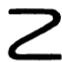
\includegraphics[keepaspectratio]{images/part001_ec6127c7.jpg}}

\begin{enumerate}
\def\labelenumi{\arabic{enumi})}
\setcounter{enumi}{1}
\item
  Let \(\mathbf{F}\) be a locally convex space, which is the union of an increasing sequence of vector subspaces \((\mathbf{F}_n)\) , and for each index \(n\) , let \(\mathcal{T}_n\) be the topology induced on \(\mathbf{F}_n\) by the topology \(\mathcal{T}\) of \(\mathbf{F}\) . One should beware that in general \(\mathcal{T}\) is not the inductive limit of the \(\mathcal{T}_n\) .
\item
  Suppose that \(\mathbf{E}\) is the strict inductive limit of the sequence \((\mathbf{E}_n)\) ; if \(\mathbf{F}\) is a closed (in \(\mathcal{T}\) ) vector subspace of \(\mathbf{E}\) , it may be the case that the strict inductive limit of the topologies induced by the \(\mathcal{T}_n\) on \(\mathrm{F} \cap \mathrm{E}_n\) is strictly finer than the topology induced by \(\mathcal{T}\) (IV, p.~63, exerc. 10).
\end{enumerate}

PROPOSITION 10. --- Let E, F be two locally convex spaces. Suppose that :

\begin{enumerate}
\def\labelenumi{\arabic{enumi})}
\item
  There exists a family of Fréchet spaces \((\mathbf{E}_{\alpha})\) , and for each \(\alpha\) a linear mapping \(g_{\alpha}: \mathbf{E}_{\alpha} \to \mathbf{E}\) , such that the topology of \(\mathbf{E}\) is the final locally convex topology for the family \((g_{\alpha})\) .
\item
  There exists a sequence of Fréchet spaces \((\mathbf{F}_n)\) and for each \(n\) a continuous linear injection \(j_n: \mathbf{F}_n \to \mathbf{F}\) such that \(\mathbf{F} = \bigcup j_n(\mathbf{F}_n)\) .
\end{enumerate}

Then every linear mapping \(u\) of \(\mathbf{E}\) in \(\mathbf{F}\) , whose graph is closed in \(\mathbf{E} \times \mathbf{F}\) , is necessarily continuous.

To prove that u is continuous, it is sufficient to show that for every \(\alpha\) , the mapping \(u \circ g_{\alpha}: E_{\alpha} \to F\) is continuous (II, p.~27, prop. 5). Now the graph of \(u \circ g_{\alpha}\) is the inverse image of the graph of u under the continuous mapping \(g_{\alpha} \times 1_{F}: E_{\alpha} \times F \to E \times F\) , and therefore is, by hypothesis, closed in \(E_{\alpha} \times F\) . We can, therefore, restrict ourselves to the case when E itself is a Fréchet space. But then the proposition is a particular case of I, p.~20, prop. 1.

COROLLARY. --- With the same hypotheses on E and F as in prop. 10 and assuming that E is Hausdorff, then every continuous surjective mapping v of F in E is a strict morphism.

Let N be the kernel of v and write \(\mathrm{N}_{n}=j_{n}^{-1}(\mathrm{N})\) ; then the mapping \(j_{n}^{\prime}:F_{n}/N_{n}\to F/N\) , deduced from \(j_{n}\) by taking quotients, is injective and continuous, also \(F_{n}/N_{n}\) is a Fréchet space (since \(N_{n}\) is closed) and F/N is the union of the images under \(j_{n}^{\prime}\) . By hypothesis, in the canonical factorisation \(v:F\to F/N\stackrel{w}{\to}E\) , the linear mapping w is bijective and continuous and its graph in \((\mathrm{F/N})\times\mathrm{E}\) is therefore closed (GT, I, §8.1, cor. 2 of prop. 2). By the remarks at the beginning and by prop. 10, the inverse mapping u of w is therefore continuous and the corollary is proved.

* Prop. 10 and its corollary apply in particular when E is a complete bornological space (III, p.~12) and F is the inductive limit of a sequence of Fréchet spaces.*

\subsection{Remarks on Fréchet spaces}

We are going to consider prop. 2 of GT, IX, § 3.1 in the case of locally convex spaces.

PROPOSITION 11. --- Let E be a metrisable locally convex space. The topology of E can be defined by a distance that is invariant under translations, and for which the open balls are convex.

Let \((p_{n})_{n\in\mathbf{N}}\) be a sequence of semi-norms that define the topology of E. Let \(d_{n}\) be the pseudometric defined by \(d_{n}(x,y)=\inf(p_{n}(x-y),1/n)\) for x,y in E; it is invariant under translations. For every \(n\geqslant0\) , and every real number \(R\geqslant0\) , let \(B_{n,R}\) be the set of \(x\in E\) for which \(d_{n}(x,0)<R\) . If \(R\geqslant1/n\) , then \(B_{n,R}=E\) , and in the other case \(B_{n,R}\) is formed from the \(x\in E\) such that \(p_{n}(x)<R\) ; in all cases \(B_{n,R}\) is convex.

For \(x, y\) in \(\mathbf{E}\) define \(d(x, y) = \sup_{n \in \mathbb{N}} d_n(x, y)\) . We see immediately that \(d\) is a distance, invariant under translations on \(\mathbf{E}\) and defining the topology of \(\mathbf{E}\) . For \(x_0 \in \mathbf{E}\) and \(\mathbf{R} \geqslant 0\) , the open ball with centre \(x_0\) and radius \(\mathbf{R}\) (for the distance \(d\) ) is equal to \(\bigcap_{n \in \mathbb{N}} (x_0 + B_{n,\mathbf{R}})\) , therefore it is convex.

PROPOSITION 12. --- Let E and F be two Fréchet spaces and u a continuous linear mapping of E on F. Then there exists a section of u that is continuous though not necessarily linear.

By prop. 11 there exists a distance d in E, invariant under translations, defining the topology of E and for which open balls are convex. Given y and \(y'\) in F, let \(\delta(y, y')\) be the distance apart of the closed sets \(u^{-1}(y)\) and \(u^{-1}(y')\) in E. As u is a strict morphism (I, p.~17, th. 1) the remark of GT, IX, §3.1 shows that \(\delta\) is a distance on F defining the topology of F. We shall construct, inductively, a sequence of continuous mappings \((s_n)_{n \in \mathbf{N}}\) of F in E satisfying the following inequalities for all \(y \in F\) :

\[
\delta (y, u (s _ {n} (y))) <   2 ^ {- n}\tag{2}
\]

\[
d \left(s _ {n} (y), s _ {n - 1} (y)\right) <   2 ^ {- n + 1} \quad (\text { only   if } n \geqslant 1).\tag{3}
\]

Suppose then that either \(n = 0\) , or \(n \geqslant 1\) and that \(s_{n-1}\) has been constructed. Let \(y_0 \in \mathbf{F}\) ; as \(u\) is surjective, the set \(u^{-1}(y_0)\) is non-empty, and for \(n \geqslant 1\) , we have \(d(u^{-1}(y_0), s_{n-1}(y_0)) < 2^{-n+1}\) by the induction hypothesis. Therefore there exists a point \(x_0\) of \(\mathbf{E}\) such that \(u(x_0) = y_0\) and for \(n \geqslant 1\) , \(d(x_0, s_{n-1}(y_0)) < 2^{-n+1}\) . As the mapping \(s_{n-1}\) is continuous, the set of points \(y\) of \(\mathbf{F}\) which satisfy the inequalities \(\delta(y, y_0) < 2^{-n}\) and \(d(x_0, s_{n-1}(y)) < 2^{-n+1}\) is an open neighbourhood of \(y_0\) . Hence there exist an open covering \((\mathrm{V}_i)_{i \in \mathbf{I}}\) of \(\mathbf{F}\) and constant mappings \(s_{n,i}\) of \(\mathbf{F}\) in \(\mathbf{E}\) which satisfy the inequalities (2) and (3) in \(\mathrm{V}_i\) where one replaces \(s_n\) by \(s_{n,i}\) . As the space \(\mathbf{F}\) is metrisable, there exists a continuous partition of unity \((f_i)_{i \in \mathbf{I}}\) , that is locally finite and subordinate to the covering \((\mathrm{V}_i)_{i \in \mathbf{I}}\) (GT, IX, § 4.5, th. 4 and § 4.4, cor. 1). For every \(y \in \mathbf{F}\) , put \(s_n(y) = \sum_{i \in \mathbf{I}} f_i(y) \cdot s_{n,i}(y)\) . The mapping \(s_n\) of \(\mathbf{F}\) in \(\mathbf{E}\) is continuous; as the open balls are convex in \(\mathbf{E}\) and in \(\mathbf{F}\) , the mapping \(s_n\) satisfies the inequalities (2) and (3) for all \(y \in \mathbf{F}\) .

From inequality (3) the mappings \(s_n: \mathrm{F} \to \mathrm{E}\) form a Cauchy sequence, for uniform convergence. As \(\mathrm{E}\) is complete, the sequence \((s_n)_{n \in \mathbb{N}}\) converges uniformly to a continuous mapping \(s: \mathrm{F} \to \mathrm{E}\) (GT, X, § 1.6); formula (2) shows that \(u \circ s\) is the identity mapping of \(\mathrm{F}\) , thus \(s\) is a continuous section of \(u\) .

COROLLARY. --- If L is a compact set in F, then there exists a compact set K in E such that \(u(\mathbf{K}) = \mathbf{L}\) .

It is sufficient to put K = s(L), where s is a continuous section of u.

Remarks. --- 1) The corollary to prop. 12 can also be deduced from th. 1 of I, p.~17 and prop. 18 of GT, IX, § 2.10.

\begin{enumerate}
\def\labelenumi{\arabic{enumi})}
\setcounter{enumi}{1}
\tightlist
\item
  We keep the notations of prop. 12. Let \(p\) be a continuous semi-norm on \(E\) ;
\end{enumerate}

for all \(y \in \mathbf{F}\) , put \(q(y) = \inf_{u(x) = y} p(x)\) , so that \(q\) is a continuous semi-norm on \(\mathbf{F}\) (II, p.~4). Let \(\phi\) be a lower semi-continuous mapping of \(F\) in the interval \([0, +\infty[\) of \(\overline{\mathbf{R}}\) . We show that there exists a continuous section \(s\) of \(u\) such that \(p \circ s < q + \phi\) .

Let \(s_0\) be a continuous section of \(u\) (prop. 12) and \(\mathbf{N}\) the kernel of \(u\) . Let \(y_0 \in \mathbf{F}\) , then there exists \(z_0 \in \mathbf{N}\) such that \(p(s_0(y_0) + z_0) < q(y_0) + \phi(y_0)\) . There exists an open neighbourhood \(\mathbf{W}\) of \(y_0\) in \(\mathbf{F}\) such that \(p(s_0(y) + z_0) < q(y) + \phi(y)\) for all \(y \in \mathbf{W}\) . Hence there is an open covering \((\mathbf{W}_i)_{i \in \mathbf{I}}\) of \(\mathbf{F}\) and constant mappings \(t_i: \mathbf{F} \to \mathbf{N}\) such that \(p(s_0(y) + t_i(y)) < q(y) + \phi(y)\) for all \(y \in \mathbf{W}_i\) . As \(\mathbf{F}\) is metrisable, there exists a locally finite continuous partition of unity subordinated to the covering \((\mathbf{W}_i)_{i \in \mathbf{I}}\) , say \((g_i)_{i \in \mathbf{I}}\) (GT, IX, § 4.5, th. 4 and § 4.4, cor. 1). The mapping \(s\) of \(\mathbf{F}\) in \(\mathbf{E}\) defined by \(s(y) = s_0(y) + \sum_{i \in \mathbf{I}} g_i(y). t_i(y)\) fulfils the stated conditions.

\section{SEPARATION OF CONVEX SETS}

\subsection{The Hahn-Banach theorem (geometric form)}

THEOREM 1 (Hahn-Banach). --- Let A be an open convex non empty set of the topological vector space E and let M be a non-empty linear variety which does not meet A. Then there exists a closed hyperplane H which contains M and does not meet A.

By translation the problem can be reduced to the case \(0 \in A\) , so that A is absorbent. Let p be the gauge of A (II, p.~20) so that A is the set of points \(x \in E\) such that \(p(x) < 1\) . On the other hand, let V be the vector subspace of E generated by M; thus M is a hyperplane in V that does not contain 0, and hence there is a unique linear form f on V such that M is the set of points \(y \in V\) for which \(f(y) = 1\) . The hypothesis \(M \cap A = \varnothing\) implies therefore that for all \(y \in V\) for which \(f(y) = 1\) , we have \(p(y) \geqslant 1\) ; as f and p are positively homogeneous we have \(f(y) \leqslant p(y)\) for all \(y \in V\) such that \(f(y) > 0\) ; finally as \(p(y) \geqslant 0\) for all \(y \in V\) , we see that \(f(y) \leqslant p(y)\) for all \(y \in V\) . By the analytical form of the Hahn-Banach theorem (II, p.~22, th. 1) there exists a linear form h on E which extends f and is such that, for all \(x \in E\) , \(h(x) \leqslant p(x)\) . Let H be the hyperplane in E with the equation \(h(x) = 1\) . Clearly \(H \cap V = M\) and \(H \cap A = \varnothing\) . On the other hand the complement of H in E contains the open non-empty set A, therefore H is closed in E (I, p.~11, corollary).

Q.E.D.

Remarks. --- 1) When \(0 \in \mathbf{M}\) , th. 1 can be stated as follows: there exists a continuous linear form in E, such that \(g(x) = 0\) in M and \(g(x) > 0\) in A (II, p.~8, prop. 4).

\begin{enumerate}
\def\labelenumi{\arabic{enumi})}
\setcounter{enumi}{1}
\tightlist
\item
  If we apply theorem 1 to the case where E carries the finest locally convex topology (II, p.~25, Example 2), and if, for the sake of simplicity, we suppose that \(0 \in A\) , then we get the following result (that superficially does not involve topology): if A is an absorbent convex set in the real vector space E and if M is a non-empty linear variety that does not meet A, then there exists a hyperplane H containing M and such that A lies on one side of H. This result is not valid for every convex set A (II, p.~65, exerc. 5).
\end{enumerate}

\subsection{Separation of convex sets in a topological vector space}

DEFINITION 1. --- Two non-empty sets A, B of a real topological vector space E are said to be separated by a closed hyperplane H if A is contained in one of the closed half-spaces determined by H and B is contained in the other closed half-space.

DEFINITION 2. --- Two non-empty sets A, B of a real topological vector space are said to be strictly separated by the closed hyperplane H if A is contained in one of the open half-spaces determined by H, and B is contained in the other open half-space.

PROPOSITION 1. --- Let A be an open non-empty convex set and let B be a non-empty convex set in a real topological vector space E; if A does not meet B then there exists a closed hyperplane that separates A from B.

For the set \(\mathbf{C} = \mathbf{A} - \mathbf{B}\) is open, convex (II, p.~9, prop. 7) and non-empty, also \(0 \notin \mathbf{C}\) . By theorem 1 of II, p.~36, there exists a continuous linear form \(f \neq 0\) on \(\mathbf{E}\) such that \(f(z) > 0\) in \(\mathbf{C}\) . Then, for all \(x \in \mathbf{A}\) , and \(y \in \mathbf{B}\) , we have \(f(x) > f(y)\) . Write \(\alpha = \inf_{x \in \mathbf{A}} f(x)\) ; \(\alpha\) is finite and we have \(f(x) \geqslant \alpha\) for all \(x \in \mathbf{A}\) and \(f(y) \leqslant \alpha\) for all \(y \in \mathbf{B}\) ; the closed hyperplane \(\mathbf{H}\) with the equation \(f(z) = \alpha\) separates \(\mathbf{A}\) from \(\mathbf{B}\) .

Remarks. --- 1) The hyperplane H does not meet A (II, p.~15, prop. 1; if A and B are two convex non-empty open sets that do not meet then there exists a closed hyperplane that separates A strictly from B.

2) However, when B is not open, it is not necessarily the case that there exists a closed hyperplane that separates A strictly from B, even if E is of finite dimension, and even if \(\overline{A}\) does not meet \(\overline{B}\) (II, p.~78, exerc. 12).

DEFINITION 3. --- For a subset A of a vector space E, a hyperplane H is called a support hyperplane of A, if H contains at least one point of A and all the points of A lie on the same side of H.

Let f be a linear form on E that is not identically zero; to say that the hyperplane of the equation \(f(x) = \alpha\) is a support hyperplane of A means that \(\alpha\) is either the smallest or the largest member of the set \(f(A) \subset R\) . In other words, there exists a support hyperplane of A parallel to the hyperplane of equation \(f(x) = 0\) , if, and only if, one of the bounds of the set \(f(A)\) is finite and belongs to \(f(A)\) .

PROPOSITION 2. --- Let A be a non-empty compact subset of a topological vector space E. For every closed hyperplane H in E, there exists a support hyperplane of A parallel to H.

For, if \(f(x) = \gamma\) is an equation of H, where f is a continuous linear form in E, the restriction of f to A is continuous, therefore bounded and attains its bounds in A (GT, IV, § 6.1, th. 1).

This demonstrates that there exist one or two support hyperplanes of A parallel to H; the first case can only arise when A is completely contained in a hyperplane parallel to H.

PROPOSITION 3. --- In a topological vector space E, let A be a closed convex set with a non-empty interior. Then every support hyperplane of \(\mathbf{A}\) is closed and every frontier point of \(\mathbf{A}\) belongs to at least one support hyperplane of \(\mathbf{A}\) .

Every support hyperplane of A is closed, since all the points of A are on the same side of the hyperplane (II, p.~15, prop. 17). Also if \(x_0\) is a frontier point of A, then \(x_0\) does not belong to the open non-empty convex set \(\mathring{\mathrm{A}}\) ; after th. 1 of II, p.~36 there exists a hyperplane H that contains \(x_0\) and does not meet \(\mathring{\mathrm{A}}\) . As A is the closure of \(\mathring{\mathrm{A}}\) (II, p.~14, cor. 1 to prop. 16), it follows from prop. 17 of II, p.~15 that H is a support hyperplane of A.

\subsection{Separation of convex sets in a locally convex space}

PROPOSITION 4. --- Let A be a closed non-empty convex set in a locally convex space E and let K be a compact non-empty convex set in E, that does not meet A. Then there exists a closed hyperplane H that strictly separates A from K.

For there exists an open convex neighbourhood V of 0 in E such that A + V and K + V do not meet (GT, II, § 4.3, prop. 4). As A + V and K + V are convex and open in E, prop. 1 of II, p.~37 shows that there exists a closed hyperplane H that strictly separates A + V from K + V, and a fortiori A from K.

Remark. --- In a Hausdorff locally convex space E, let A and B be two closed non-empty convex sets that are disjoint, if E is finite dimensional then there exists a closed hyperplane that separates A from (II, p.~78, exerc. 13); but this conclusion is not necessarily true when E is of infinite dimension (II, p.~78, exerc. 10 and 11).

COROLLARY 1. --- In a locally convex space, every closed convex set A is the intersection of the closed half-spaces which contain it.

In fact, for every point \(x \notin \mathbf{A}\) , there exists a closed hyperplane that separates \(x\) strictly from \(\mathbf{A}\) (using prop. 4).

COROLLARY 2. --- In a Hausdorff locally convex space, every compact convex set A is the intersection of the closed half-spaces which contain it and which are determined by support hyperplanes of A.

For, let \(x_{0} \notin A\) ; \(\{x_{0}\}\) is closed, therefore there exists a closed hyperplane H which separates \(x_{0}\) strictly from A (prop. 4); let \(f(x) = \alpha\) be an equation of H (f a continuous linear form) and suppose that \(f(x) > \alpha\) for all \(x \in A\) . If we put \(\gamma = \inf_{x \in A} f(x)\) , the half-space defined by \(f(x) \geqslant \gamma\) contains A, is determined by the support hyperplane of equation \(f(x) = \gamma\) , and does not contain \(x_{0}\) ; whence the corollary.

It is possible that a closed convex set that is not compact and has no interior point, in a locally convex space, does not have any closed support hyperplane (II, p.~86, exerc. 18 : cf.~also V, p.~71, exerc. 11).

COROLLARY 3. --- In a locally convex space, the closure of each linear variety M is the intersection of the closed hyperplanes that contain M.

For all \(x \notin \overline{\mathbf{M}}\) , let \(\mathbf{H}\) be a closed hyperplane that separates \(x\) strictly from \(\overline{\mathbf{M}}\) ;

thus \(\overline{M}\) is parallel to H; the closed hyperplane \(H_{1}\) , containing \(\overline{M}\) and parallel to H does not contain x. The corollary follows.

COROLLARY 4. --- Let C be a closed convex set in a locally convex space E. A subset A of E is contained in C, if, and only if, for every real valued continuous affine function u in E such that \(u(x) \geqslant 0\) for all x in C, we have \(u(y) \geqslant 0\) for all y in A.

The condition is obviously necessary. Conversely we show that it is sufficient; if a point \(x \in A\) is not contained in C, there exists a closed hyperplane of equation \(f(z) = \alpha\) separating x strictly from C; if we suppose for example that \(f(x) < \alpha\) , then the continuous affine function \(u = f - \alpha\) contradicts the hypotheses.

COROLLARY 5. --- In a locally convex space E, the closure of each convex cone C of vertex 0 is the intersection of closed half-spaces containing C determined by closed hyperplanes that pass through 0.

For \(\overline{\mathbf{C}}\) is a convex cone of vertex 0 (II, p.~13, prop. 14). For \(x \notin \overline{\mathbf{C}}\) , there exists a closed hyperplane H that separates \(x\) strictly from \(\overline{\mathbf{C}}\) (prop. 4). It is now just necessary to apply the following lemma:

Lemma 1. --- If a cone A, with vertex 0, is contained in an open half-space determined by a hyperplane H, then it is contained in a closed half-space determined by a hyperplane \(H_{0}\) , that is parallel to H and passes through 0.

Let \(f(z) = \alpha\) with \(\alpha < 0\) be an equation of H, so that \(f(z) = 0\) is the equation of \(H_0\) . If there exists \(z \in A\) such that \(f(z) < 0\) , then there would exist \(\lambda > 0\) , such that \(f(\lambda z) = \alpha\) , and as \(\lambda z \in A\) , this would contradict the hypothesis.

\subsection{Approximation to convex functions}

PROPOSITION 5. --- Let X be a closed convex set in a locally convex space E. Then every lower semi-continuous convex function f defined in X is the upper envelope of a family of functions that are the restrictions to X of continuous affine linear functions in E.

For, the set \(A \subset E \times R\) of points \((x, t)\) such that \(x \in X\) and \(t \geqslant f(x)\) is convex (II, p.~17, prop. 19) and closed, since the function \((x, t) \mapsto f(x) - t\) is lower semicontinuous. Then let x be any point of X and let \(a \in R\) be such that \(a < f(x)\) . By cor. 1 of II, p.~38, there exists a closed hyperplane H in \(E \times R\) , that contains \((x, a)\) and does not meet A. Every linear continuous form on \(E \times R\) being of the form

\[
(z, t) \rightarrow u (z) + \lambda t,
\]

where \(\lambda\in R\) and u is a continuous linear form on E, it follows that H has an equation of the form \(u(z)+\lambda t=\alpha\) , and as H contains \((x,a)\) we have \(\alpha=u(x)+\lambda a\) . Now the point \((x,f(x))\in\mathbf{A}\) does not belong to H and therefore \(\lambda\neq0\) . Dividing by \(-\lambda\) , if necessary, we can write the equation of H as \(t-a=u(z-x)\) . As \(f(x)-a>0\) , we have, therefore, \(f(z)>u(z-x)+a\) for all \(z\in X\) and this proves the proposition.

Remarks. --- 1) It follows from prop. 5 that f is the upper envelope of a directed increasing family of functions that are the restrictions to X of functions which are continuous and convex in E.

\begin{enumerate}
\def\labelenumi{\arabic{enumi})}
\setcounter{enumi}{1}
\tightlist
\item
  Suppose further that X is a closed convex cone with vertex 0 and that f is positively homogeneous. Then f is the upper envelope of a family of functions which are the restrictions to X of continuous linear forms in E. For, let \((u_{\alpha})\) be a family of continuous affine linear functions in E of which the restrictions to X have f as their upper envelope. Put \(u_{\alpha} = v_{\alpha} + \lambda_{\alpha}\) , where \(\lambda_{\alpha} \in R\) , and where \(v_{\alpha}\) is a continuous linear form in E. We have \(\lambda_{\alpha} = u_{\alpha}(0) \leqslant f(0) = 0\) . On the other hand, if \(x \in X\) , we have for every \(\mu > 0\) ,
\end{enumerate}

\[
\mu^ {- 1} \lambda_ {\alpha} + v _ {\alpha} (x) = \mu^ {- 1} (\lambda_ {\alpha} + v _ {\alpha} (\mu x)) = \mu^ {- 1} u _ {\alpha} (\mu x) \leqslant \mu^ {- 1} f (\mu x) = f (x)
\]

therefore \(u_{\alpha} \leqslant v_{\alpha} \leqslant f\) in X so that \(f\) is the upper envelope of the \(v_{\alpha}\) .

\begin{enumerate}
\def\labelenumi{\arabic{enumi})}
\setcounter{enumi}{2}
\tightlist
\item
  The restriction to X of a continuous affine function in E is a function that is affine in X (i.e.~both concave and convex II, p.~17); but it may be the case that there exist continuous affine functions in a compact convex set \(\mathbf{X} \subset \mathbf{E}\) , that are not the restrictions to X of continuous affine functions in E (II, p.~78, exerc. II, c)). However:
\end{enumerate}

PROPOSITION 6. --- Let f be an upper semi-continuous affine function in a compact convex set X, of the Hausdorff locally convex space E. Let L be the set of restrictions to X of continuous affine functions in E; the set L' of the \(h \in L\) such that \(h(x) > f(x)\) for all \(x \in X\) , is then decreasing directed and its lower envelope is equal to f.

We may suppose that X is non-empty. Let u, v be two elements of L, such that \(u(x) > f(x)\) and \(v(x) > f(x)\) for all \(x \in X\) , and let b be a constant that is an upper bound of u and v. Let U (resp. V) be the compact convex set of points \((x, t)\) of \(X \times R\) such that \(u(x) \leqslant t \leqslant b\) (resp. \(v(x) \leqslant t \leqslant b\) ), and let F be the set of \((x, t) \in X \times R\) such that \(t \leqslant f(x)\) ; F is convex and closed in \(X \times R\) . The convex envelope K of \(U \cup V\) does not meet F, since \(U \cup V\) is contained in the set of \((x, t) \in X \times R\) such that \(f(x) < t\) , a set which is convex and does not meet F. As K is compact (II, p.~14, prop. 15), we can separate F strictly from K by a closed hyperplane H in \(E \times R\) . For every \(x \in X\) , the hyperplane H separates \((x, f(x))\) strictly from \((x, b)\) , and therefore meets the line \(\{x\} \times R\) in a single point \(w(x)\) ; thus H is the graph of a continuous affine function whose restriction w to X is a member of L, that is a lower bound for u and v and that satisfies the inequality \(w(x) > f(x)\) for all \(x \in X\) . This proves that the set \(L'\) is decreasing directed. Prop. 5 of II, p.~39, applied to -f shows that f is the lower envelope of \(L'\) .

COROLLARY. --- Let \(f\) be a continuous affine function in \(\mathbf{X}\) ; then there exists a sequence \((h_n)\) of elements of \(\mathbf{L}\) which converges uniformly to \(f\) in \(\mathbf{X}\) .

For, prop. 6 and Dini's theorem (GT, X, § 4.1, th. 1) show that for all \(n\) there exists \(h_n \in \mathbf{L}\) such that \(f \leqslant h_n \leqslant f + 1/n\) .

\section{WEAK TOPOLOGIES}

\subsection{Dual vector spaces}

Let \(\mathbf{F}\) and \(\mathbf{G}\) be two real vector spaces and let \((x, y) \mapsto \mathbf{B}(x, y)\) be a bilinear form on \(\mathbf{F} \times \mathbf{G}\) . We say that the bilinear form \(\mathbf{B}\) puts the vector spaces \(\mathbf{F}\) and \(\mathbf{G}\) in duality, or that F and G are in duality (relative to B). Recall that we say that \(x \in F\) and \(y \in G\) are orthogonal (for the duality defined by B) if \(\mathbf{B}(x, y) = 0\) ; we say that a subset M of F and a subset N of G are orthogonal if every \(x \in M\) is orthogonal to every \(y \in N\) (A, IX, § 1.2).

We say that the duality defined by B is separating in F (resp. in G) if it satisfies the following condition :

(D₁) For every \(x \neq 0\) in F, there exists \(y \in G\) such that \(\mathrm{B}(x, y) \neq 0\) . (resp. (D \(_{II}\) ) For every y ≠ 0 in G, there exists x ∈ F such that B(x, y) ≠ 0.)

The duality defined by B is said to be separating if it is both separating in F and in G. For this to be so, it is necessary and sufficient that the bilinear form B should be separating in the sense of A, IX, § 1.1. More precisely we have the following result:

PROPOSITION 1. --- Let F, G be two real vector spaces and B a bilinear form on F × G. Let

\[
d _ {\mathrm{B}}: y \mapsto \mathrm{B} (., y),
\]

\[
s _ {\mathbf {B}} \colon x \mapsto \mathrm{B} (x,.)
\]

be linear mappings of G in the dual F* of F and of F in the dual G* of G, associated respectively to the right and to the left of B (A, IX, § 1.1). Then B puts F and G in a duality separating in G (resp. in F), if and only if \(d_{\mathbf{B}}\) (resp. \(s_{\mathbf{B}}\) ) is injective.

When F and G are put in separating duality by B, we often identify F (resp. G) with a subspace of \(G^{*}\) (resp. \(F^{*}\) ) by means of \(s_{B}\) (resp. \(d_{B}\) ). When we consider F (resp. G) as a subspace of \(G^{*}\) (resp. \(F^{*}\) ) without specifying how this identification is to be made, we are always using the preceding identifications; the bilinear form B is then identified with the restriction to \(F \times G\) of the canonical bilinear form:

\[
(x ^ {*}, x) \mapsto \langle x, x ^ {*} \rangle \quad (\text { resp. } (x, x ^ {*}) \mapsto \langle x, x ^ {*} \rangle).
\]

Examples. --- 1) Let E be a vector space and let E* be its dual. The canonical bilinear form \((x, x^{*}) \mapsto \langle x, x^{*} \rangle\) on \(E \times E^{*}\) (A, II, §2.3) puts E and \(E^{*}\) in separating duality: for \((\mathrm{D}_{\mathrm{II}})\) is true because of the definition of the relation \(x^{*} \neq 0\) , and we know on the other hand, that for all \(x \neq 0\) in E, there exists a linear form \(x^{*} \in E^{*}\) such that \(\langle x, x^{*} \rangle \neq 0\) (A, II, §7.5, th. 6), which proves \((\mathrm{D}_{\mathrm{I}})\) ; the identifications of E with a subspace of \(E^{**}\) is made here by the canonical mapping \(c_{E}\) (loc. cit.).

When E is of finite dimension, the only subspace G of \(E^{*}\) that is in separating duality by the restriction to \(E \times G\) of the canonical bilinear form, is the space \(E^{*}\) itself; for, E being then canonically identified with \(E^{**}\) (loc. cit.), if we had \(G \neq E^{*}\) , there would exist \(a \neq 0\) in E such that \(\langle a, x^{*} \rangle = 0\) for all \(x^{*} \in G\) (A, II, §7.5, th. 7), which contradicts the hypothesis.

\begin{enumerate}
\def\labelenumi{\arabic{enumi})}
\setcounter{enumi}{1}
\tightlist
\item
  When E is an infinite dimensional vector space, and \(E'\) is a vector subspace of \(E^{*}\) , the duality between E and \(E'\) defined by the restriction to \(E \times E'\) of the canonical bilinear form is always separating in \(E'\) ; it can be separating in E even if \(E' \neq E^{*}\) . The most important case occurs where E is a topological vector space.
\end{enumerate}

DEFINITION 1. --- By the dual of a topological vector space E, we mean the subspace E' of E*, the dual of the vector space E, formed by the continuous linear forms on E.

When E is a Hausdorff locally convex space, the duality between E and its dual \(E'\) is separating: this follows from the Hahn-Banach theorem (II, p.~24, cor. 1) that for every \(x \neq 0\) in E, there exists \(x' \in E'\) such that \(\langle x, x' \rangle \neq 0\) .

Remarks. --- 1) When E is a topological vector space, the dual E* of the vector space E will be called the algebraic dual of E to avoid confusion. We note also that E* is the dual of the topological vector space obtained by giving E the finest locally convex topology (II, p.~25, Example 2).

\begin{enumerate}
\def\labelenumi{\arabic{enumi})}
\setcounter{enumi}{1}
\item
  The dual \(\mathbf{E}'\) of a topological vector space does not itself carry a topology, unless this is expressly stated.
\item
  If \(\mathbf{F}\) and \(\mathbf{G} \subset \mathbf{F}^*\) are in separating duality by the canonical bilinear form, then this is also true of \(\mathbf{F}\) and \(\mathbf{G}_1\) , for every subspace \(\mathbf{G}_1\) of \(\mathbf{F}^*\) such that \(\mathbf{G} \subset \mathbf{G}_1\) .
\end{enumerate}

\subsection{Weak topologies}

DEFINITION 2. --- Let F and G be two vector spaces put in duality by the bilinear form B. The coarsest topology on F that makes all the linear forms \(\mathbf{B}(., y): x \mapsto \mathbf{B}(x, y)\) continuous, where y varies in G, is called the weak topology on F defined by the duality between F and G, and we denote it by \(\sigma(\mathbf{F}, \mathbf{G})\) .

Similarly we define the weak topology \(\sigma(\mathbf{G},\mathbf{F})\) on \(\mathbf{G}\) , interchanging \(\mathbf{F}\) and \(\mathbf{G}\) in definition 1; this possibility of interchanging \(\mathbf{F}\) and \(\mathbf{G}\) applies to all the results and definitions that follow in this paragraph.

We use the adjective « weak » and the adverb « weakly » to denote properties relative to a weak topology \(\sigma(\mathrm{F},\mathrm{G})\) provided there is no possibility of confusion. We shall speak, for example, of « weak convergence » and « weakly continuous functions » etc.

When \(G \subset F^{*}\) , the notation \(\sigma(F, G)\) will always denote the weak topology defined by the duality corresponding to the restriction to \(F \times G\) of the canonical bilinear form \((x, x^{*}) \mapsto \langle x, x^{*} \rangle\) .

Without extra hypotheses on F and G, we often write \(\langle x, y \rangle\) for the value \(\mathbf{B}(x, y)\) of the bilinear form B at \((x, y)\) , provided there is no ambiguity; we shall adopt this convention in the rest of this paragraph.

A vector space F carrying a weak topology of \(\sigma(F, G)\) will be called a weak space. A weak topology \(\sigma(F, G)\) is locally convex (II, p.~26, prop. 4); more precisely, it is the inverse image of the product topology of \(\mathbf{R}^G\) by the linear mapping \(\phi: x \mapsto (\langle x, y \rangle)_{y \in G}\) of \(F\) in \(\mathbf{R}^G\) . It is defined by the set of semi-norms \(x \mapsto |\langle x, y \rangle|\) when \(y\) varies in \(G\) (II, p.~5). For every \(\alpha > 0\) , and every finite family \((y_i)_{1 \leq i \leq n}\) of points of \(G\) , let \(W(y_1, ..., y_n; \alpha)\) be the set of the \(x \in F\) such that \(|\langle x, y_i \rangle| \leqslant \alpha\) for \(1 \leq i \leq n\) ; these sets (for \(\alpha, n\) and \(y_i\) arbitrary) form a fundamental system of neighbourhoods of 0 for \(\sigma(F, G)\) . Note that \(W(y_1, ..., y_n; \alpha)\) contains that vector subspace of \(F\) , of finite codimension, which is defined by the equations \(\langle x, y_i \rangle = 0\) for \(1 \leq i \leq n\) .

PROPOSITION 2. --- The weak topology \(\sigma(F, G)\) is Hausdorff if and only if the duality between \(F\) and \(G\) is separating in \(F\) .

This is a particular case of II, p.~3, prop. 2.

PROPOSITION 3. --- Let F and G be two real vector spaces in duality. Every linear form on F, that is continuous for \(\sigma(F, G)\) , can be written as \(x \mapsto \langle x, y \rangle\) for some \(y \in G\) . The element \(y \in G\) is unique when the duality is separating in G.

For, to say that the linear form \(f\) on \(\mathbf{F}\) is continuous for \(\sigma(\mathbf{F}, \mathbf{G})\) means that there exists a finite set of points \(y_i \in \mathbf{G}\) ( \(1 \leqslant i \leqslant n\) ) such that, for all \(x\) in \(\mathbf{F}\) , \(|f(x)| \leqslant \sup_{1 \leqslant i \leqslant n} |\langle x, y_i \rangle|\) (II, p.~6, prop. 5). The \(n\) relations \(\langle x, y_i \rangle = 0\) ( \(1 \leqslant i \leqslant n\) ) imply therefore \(f(x) = 0\) , and hence (A, II, § 7.5, cor. 1), there exists a linear combination \(y = \sum_{i=1}^{n} \lambda_i y_i\) such that \(f(x) = \langle x, y \rangle\) for all \(x \in \mathbf{F}\) . The uniqueness follows from \((\mathrm{D}_{\mathrm{II}})\) .

In other words, when the duality is separating in G, and F has the topology \(\sigma(\mathrm{F}, \mathrm{G})\) , then we can identify G canonically with the dual of F for this topology (II, p.~42, def. 1).

COROLLARY 1. --- A family \((a_i)\) of points of F is total for the topology \(\sigma(\mathrm{F},\mathrm{G})\) if, and only if, for every \(y \neq 0\) in G, there exists an index \(\iota\) such that \(\langle a_{\iota}, y \rangle \neq 0\) .

For using prop. 3 and I, p.~13, th. 1, the property expresses the fact that for \(\sigma(F, G)\) no closed hyperplane contains all the \(a_{i}\) ; the corollary follows therefore from cor. 3 of II, p.~38.

COROLLARY 2. --- A family \((a_{\iota})\) of points of F is topologically independent for the topology \(\sigma(\mathrm{F}, \mathrm{G})\) , if, and only if, for every index \(\iota\), there exists an element \(b_{\iota} \in G\) such that: \(\langle a_{\iota}, b_{\iota} \rangle \neq 0\) and \(\langle a_{\kappa}, b_{\iota} \rangle = 0\) for all \(\kappa \neq \iota\) .

This means, that for all \(\iota\) , there exists a closed hyperplane in \(\sigma(F, G)\) , which contains all the \(a_{\kappa}\) with index \(\kappa \neq \iota\) but does not contain \(a_{\iota}\) .

COROLLARY 3. --- Let \(G_{1}\) and \(G_{2}\) be two vector subspaces of \(F^{*}\) , in duality with F (for the restriction of the canonical bilinear form). Then \(\sigma(F, G_{2})\) is finer than \(\sigma(F, G_{1})\) if and only if \(G_{1} \subset G_{2}\) .

The condition is obviously sufficient; conversely, if \(\sigma(F, G_2)\) is finer than \(\sigma(F, G_1)\) , then every linear form that is continuous for \(\sigma(F, G_1)\) is also continuous for \(\sigma(F, G_2)\) , hence \(G_1 \subset G_2\) by prop. 3.

COROLLARY 4. --- Let G be a vector subspace of the dual F*, of the vector space F. Then F and G are in separating duality (for the canonical bilinear form) if, and only if, G is dense in F* in the topology σ(F*, F).

This follows from cor. 1.

\subsection{Polar sets and orthogonal subspaces}

DEFINITION 2. --- Let F and G be two (real) vector spaces in duality. For every set M of F we call the polar of M, the set of those \(y \in G\) for which \(\langle x, y \rangle \geqslant -1\) for all \(x \in M\) . (For complex vector spaces, cf.~II, p.~64.)

If \(G_{1}\) , \(G_{2}\) are two subspaces of \(F^{*}\) such that \(G_{1} \subset G_{2}\) , then the polar of M in \(G_{1}\) is the intersection of \(G_{1}\) with the polar of M in \(G_{2}\) .

When there is no danger of confusion we use \(M^{\circ}\) to denote the polar, in G, of the subset M of F. Similarly we define the polar in F of a set in G.

Obviously, for every scalar \(\lambda \neq 0\) and all \(\mathbf{M} \subset \mathbf{F}\) , we have \((\lambda \mathbf{M})^{\circ} = \lambda^{-1} \mathbf{M}^{\circ}\) . The relation \(\mathbf{M} \subset \mathbf{N} \subset \mathbf{F}\) implies \(\mathbf{N}^{\circ} \subset \mathbf{M}^{\circ}\) ; if \(\mathbf{N}\) absorbs \(\mathbf{M}\) then \(\mathbf{M}^{\circ}\) absorbs \(\mathbf{N}^{\circ}\) ; for every family \((\mathbf{M}_{\alpha})\) of sets of \(\mathbf{F}\) , the polar set of \(\bigcup_{\alpha} \mathbf{M}_{\alpha}\) is the intersection of the polar sets \(\mathbf{M}_{\alpha}^{\circ}\) . Since, for \(y \in \mathbf{M}^{\circ}\) , the closed half-spaces defined by the relations \(\langle x, y \rangle \geqslant -1\) contain 0 and \(\mathbf{M}\) , we see that if \(\mathbf{M}_{1}\) is the convex envelope of \(\mathbf{M} \cup \{0\}\) , then \(\mathbf{M}_{1}^{\circ} = \mathbf{M}^{\circ}\) .

Clearly \(\mathbf{M} \subset \mathbf{M}^{\circ \circ}\) . Hence

\[
(\mathbf {M} ^ {\circ \circ}) ^ {\circ} \subset \mathbf {M} ^ {\circ} \subset (\mathbf {M} ^ {\circ}) ^ {\circ \circ} = (\mathbf {M} ^ {\circ \circ}) ^ {\circ}
\]

i.e.~\(\mathbf{M}^{\circ \circ \circ} = \mathbf{M}^{\circ}\) (cf.~S, III, § 1.5, prop. 2).

If \(\mathbf{M}\) is a symmetric subset of \(\mathrm{F}\) , \(\mathbf{M}^{\circ}\) is a symmetric subset of \(\mathbf{G}\) ; \(\mathbf{M}^{\circ}\) is also in this case the set of \(y \in \mathbf{G}\) such that \(|\langle x, y \rangle| \leqslant 1\) for all \(x \in \mathbf{M}\) .

PROPOSITION 4. --- (i) For any set M of F, the polar set \(\mathbf{M}^{\circ}\) is a convex set that contains 0 and is closed in G for the topology \(\sigma(\mathbf{G},\mathbf{F})\) .

\begin{enumerate}
\def\labelenumi{(\roman{enumi})}
\setcounter{enumi}{1}
\item
  If \(\mathbf{M}\) is a cone of vertex 0, then \(\mathbf{M}^{\circ}\) is a cone of vertex 0 and it is also the set of \(y\in \mathbf{G}\) such that \(\langle x,y\rangle \geqslant 0\) for all \(x\in \mathbf{M}\) .
\item
  If \(\mathbf{M}\) is a vector subspace of \(\mathbf{F}\) , then \(\mathbf{M}^{\circ}\) is a vector subspace of \(\mathbf{G}\) , and it is also the set of \(y \in \mathbf{G}\) such that \(\langle x, y \rangle = 0\) for all \(x \in \mathbf{M}\) .
\item
  Since the linear forms \(y \mapsto \langle x, y \rangle\) are continuous for \(\sigma(\mathbf{G}, \mathbf{F})\) the statement follows immediately from the definitions and the fact that a half-space determined by a hyperplane is convex.
\item
  If \(\mathbf{M}\) is a cone with vertex 0 and if \(x \in \mathbf{M}\) , \(y \in \mathbf{M}^{\circ}\) , then as \(\lambda x \in \mathbf{M}\) , for all \(\lambda > 0\) , we have \(\langle \lambda x, y \rangle \geqslant -1\) , i.e.~\(\lambda \langle x, y \rangle \geqslant -1\) . Since this holds for all \(\lambda > 0\) , it follows that \(\langle x, y \rangle \geqslant 0\) , and (ii) is proved.
\item
  Similarly, if \(\mathbf{M}\) is a vector subspace of \(\mathbf{F}\) , the relations \(x \in \mathbf{M}\) , \(y \in \mathbf{M}^{\circ}\) imply, this time, that \(\lambda \langle x, y \rangle \geqslant -1\) for all real \(\lambda\) which is possible only if \(\langle x, y \rangle = 0\) .
\end{enumerate}

If \(\mathbf{M}\) is a vector subspace of \(\mathbf{F}\) we say that \(\mathbf{M}^{\circ}\) is the orthogonal of \(\mathbf{M}\) in \(\mathbf{G}\) ; if \(\mathbf{G} \subset \mathbf{F}^{*}\) , then \(\mathbf{M}^{\circ}\) is the intersection of \(\mathbf{G}\) , and of the subspace orthogonal to \(\mathbf{M}\) in the algebraic dual \(\mathbf{F}^{*}\) of \(\mathbf{F}\) (A, II, § 2.4, def. 4).

For a vector subspace M of F and a vector subspace N of G we say that M and N are orthogonal if \(M \subset N^{0}\) (or, equivalently, if \(N \subset M^{\circ}\) ).

THEOREM 1 (The bipolar theorem). --- Let F, G be two real vector spaces in duality. For every subset M of F the polar set \(M^{\circ\circ}\) in F of the polar set \(M^{\circ}\) of M in G is the closed convex envelope (for \(\sigma(F, G)\) ) of \(M \cup \{0\}\) .

We have seen that we need only consider the case where M is convex and \(0 \in M\) . Denote the closure, in topology \(\sigma(F, G)\) of M by \(\overline{M}\) , then \(\overline{M}\) is a convex set in F; prop. 4 of II, p.~44 shows that \(M^{\circ\circ} \supset \overline{M}\) . On the other hand if \(a \in F\) does not belong to \(\overline{M}\) then there exists a closed hyperplane H in F which separates a strictly from \(\overline{M}\) (II, p.~38, prop. 4); since H does not contain 0, there exists \(y \in G\) such that H has the equation \(\langle x, y \rangle = -1\) (II, p.~43, prop. 3); thus \(\langle x, y \rangle > -1\) for all \(x \in \overline{M}\) and \(\langle a, y \rangle < -1\) . This implies that \(y \in M^{\circ}\) and \(a \notin M^{\circ\circ}\) , and the relation \(M^{\circ\circ} = \overline{M}\) follows.

COROLLARY 1. --- For any family \((\mathbf{M}_{\alpha})\) of closed convex sets of F (in the topology \(\sigma(\mathrm{F}, \mathrm{G})\) ), each containing 0, the polar set of the intersections \(M = \bigcap_{\alpha} M_{\alpha}\) is the convex closed envelope (for \(\sigma(\mathrm{G}, \mathrm{F})\) ) of the union of the \(M_{\alpha}^{\circ}\) .

For, if N is this convex closed envelope, then

\[
\mathbf {N} ^ {\circ} = \bigcap_ {\alpha} \mathbf {M} _ {\alpha} ^ {\circ \circ} = \bigcap_ {\alpha} \mathbf {M} _ {\alpha} = \mathbf {M}
\]

whence \(N = N^{\circ\circ} = M^{\circ}\) .

The conclusion of cor. 1 does not necessarily hold if the \(M_{\alpha}\) are not convex.

COROLLARY 2. --- For every vector subspace M of F, the subspace \(M^{\circ\circ}\) is the closure of M in the topology \(\sigma(\mathrm{F}, \mathrm{G})\) .

Remark. --- Every neighbourhood of 0 in G in the topology \(\sigma(\mathrm{G},\mathrm{F})\) contains a neighbourhood V defined by a finite number of inequalities of the form \(|\langle x_i,y\rangle |\leqslant 1\) ( \(1\leqslant i\leqslant n\) ), where the \(x_{i}\) are arbitrary points of F. If A is the symmetric convex envelope of the set of the \(x_{i}\) , then V is the polar set \(\mathrm{A}^{\circ}\) of A in G. We can say that the polars in G of finite symmetric sets in F (or of their convex envelopes) form a fundamental system of neighbourhoods of 0 in G for \(\sigma(\mathrm{G},\mathrm{F})\) . If the duality is separating in F, these convex envelopes are compact for \(\sigma(\mathrm{F},\mathrm{G})\) (II, p.~14, cor. 1 of prop. 15), and of finite dimensions. Conversely every compact, convex set of finite dimension C in F (with the \(\sigma(\mathrm{F},\mathrm{G})\) topology) is contained in the convex envelope of a finite subset of F. For, let M be a vector subspace of finite dimension containing C. If \((e_i)_{1\leqslant i\leqslant n}\) is a basis of M, we can suppose that C is contained in the closed parallelotope centre 0 and constructed on the vectors of the basis \(e_i\) (GT, VI, § 1.3); now it is immediate that this parallelotope is the convex envelope of the points \(\sum_{i=1}^{n} \varepsilon_i e_i\) with \(\varepsilon_i = \pm 1\) .

Thus we can say that (if \(\sigma(\mathrm{F},\mathrm{G})\) is Hausdorff) the polars of finite dimensional, convex, compact sets in F (for \(\sigma(\mathrm{F},\mathrm{G})\) or for any Hausdorff locally convex topology finer than \(\sigma(\mathrm{F},\mathrm{G})\) on F) form a fundamental system of neighbourhoods of 0 for \(\sigma(\mathrm{G},\mathrm{F})\) .

COROLLARY 3. --- Let T be the topology of a locally convex space E and let E' be its dual (II, p.~42, def. 1).

\begin{enumerate}
\def\labelenumi{(\roman{enumi})}
\item
  The closed convex sets in \(\mathbf{E}\) are the same for the topology \(\mathcal{T}\) and for the weak topology \(\sigma (\mathrm{E},\mathrm{E}^{\prime})\) .
\item
  For every subset \(\mathbf{M}\) of \(\mathbf{E}\) , the polar set \(\mathbf{M}^{\circ \circ}\) in \(\mathbf{E}\) of the polar set \(\mathbf{M}^{\circ}\) of \(\mathbf{M}\) in \(\mathbf{E}'\) , is the convex closed envelope of \(\mathbf{M} \cup \{0\}\) for the topology \(\mathcal{T}\) .
\end{enumerate}

Clearly, (ii) follows from (i) and th. 1. From the definition of the dual E', it follows from II, p.~43, prop. 3 that the continuous linear forms on E for the topology T are the same as the continuous linear forms for \(\sigma(\mathrm{E}, \mathrm{E}')\) . The closed half-spaces in E are therefore the same for T and for \(\sigma(\mathrm{E}, \mathrm{E}')\) (II, p.~15, prop. 17) and the assertion (i) follows therefore from II, p.~38, cor. 1.

\subsection{Transposition of a continuous linear mapping}

In this No., we suppose that \((\mathrm{F},\mathrm{G})\) and \((\mathrm{F}_1,\mathrm{G}_1)\) are two vector spaces in duality.

PROPOSITION 5. --- Let u be a linear mapping of F in \(F_{1}\) . The following properties are equivalent :

\begin{enumerate}
\def\labelenumi{\alph{enumi})}
\item
  \(u\) is continuous for the weak topologies \(\sigma (\mathrm{F},\mathrm{G})\) and \(\sigma (\mathrm{F}_1,\mathrm{G}_1)\) ;
\item
  there exists a mapping \(v: \mathbf{G}_1 \to \mathbf{G}\) such that
\end{enumerate}

\[
\langle u (y), z _ {1} \rangle = \langle y, v (z _ {1}) \rangle\tag{1}
\]

for all \(y \in \mathbf{F}\) and \(z \in \mathbf{G}_1\) .

If these properties hold and if the duality between \(\mathbf{F}\) and \(\mathbf{G}\) is separating in \(\mathbf{G}\) , then the mapping \(v\) satisfying (1) is unique, and \(v\) is linear.

If u is continuous for the weak topologies, then, for all \(z_{1} \in G_{1}\) , the linear form \(y \mapsto \langle u(y), z_{1} \rangle\) on F is continuous for \(\sigma(F, G)\) , thus (II, p.~43, prop. 3) can be written as \(y \mapsto \langle y, v(z_{1}) \rangle\) with \(v(z_{1}) \in G\) , which shows that a) implies b). Conversely, if b) is true, for all \(z_{1} \in G_{1}\) , the linear form

\[
y \mapsto \langle y, v (z _ {1}) \rangle = \langle u (y), z _ {1} \rangle
\]

is continuous for \(\sigma(\mathrm{F},\mathrm{G})\) : it follows from the definition of weak topologies that \(u\) is continuous for \(\sigma(\mathrm{F},\mathrm{G})\) and \(\sigma(\mathrm{F}_1,\mathrm{G}_1)\) (I, p.~10, cor. 1). The uniqueness of \(v\) follows from \((\mathrm{D}_{\mathrm{II}})\) and this uniqueness implies that \(v\) is linear.

Remark. --- Suppose that the duality between F and G is separating in G and that the duality between \(F_{1}\) and \(G_{1}\) is separating in \(G_{1}\) . If we identify G and \(G_{1}\) with subspaces of \(F^{*}\) and \(F_{1}^{*}\) respectively, the conditions a) and b) are equivalent to \(^{t}u(\mathbf{G}_{1}) \subset \mathbf{G}\) ; v is the restriction of the transpose \(^{t}u\) of u (A, II, §2.5) to \(G_{1}\) .

We say, simply (when there is no chance of confusion) that v is the transpose of u (relative to the duality on the one hand between F and G and on the other hand between \(F_{1}\) and \(G_{1}\) ) and we again use \(^{t}u\) to denote it.

COROLLARY. --- Suppose that the duality between F and G is separating in G. If u is a linear mapping of F in \(F_{1}\) , that is continuous for \(\sigma(F, G)\) and \(\sigma(F_{1}, G_{1})\) , then its transpose is a linear mapping of \(\mathbf{G}_1\) in \(\mathbf{G}\) , that is continuous for \(\sigma (\mathbf{G}_1,\mathbf{F}_1)\) and \(\sigma (\mathbf{G},\mathbf{F})\) . Further if the duality between \(\mathbf{F}_1\) and \(\mathbf{G}_1\) is separating in \(\mathbf{F}_1\) then \(^{t}(^{t} u) = u\) .

It is sufficient to exchange F and \(F_{1}\) with G and \(G_{1}\) in prop. 5.

PROPOSITION 6. --- Suppose that the duality between F and G (resp. \(F_{1}\) and \(G_{1}\) ) is separating in G (resp. \(F_{1}\) ). Let u be a linear mapping of F in \(F_{1}\) that is continuous for \(\sigma(F, G)\) and \(\sigma(F_{1}, G_{1})\) . Let A be a set in F and \(A_{1}\) a set in \(F_{1}\) ; then :

\begin{enumerate}
\def\labelenumi{(\roman{enumi})}
\item
  We have \((u(\mathbf{A}))^{\circ} = ({}^{t} u)^{-1} (\mathbf{A}^{\circ})\) .
\item
  We have \(\overline{{}^{t}u(A_1^\circ)}\subset (u^{-1}(A_1))^{\circ}\) ; further, if \(A_1\) is closed, (for \(\sigma(F_1,G_1)\) ) convex, and contains the origin, then we have \(\overline{{}^{t}u(A_1^\circ)} = (u^{-1}(A_1))^{\circ}\) .
\end{enumerate}

Let \(z_{1} \in G_{1}\) , the relation \(z_{1} \in (u(A))^{\circ}\) is equivalent to \(\langle u(y), z_{1} \rangle \geqslant -1\) for all \(y \in A\) , and the relation \({}^{t}u(z_{1}) \in A^{\circ}\) is equivalent to \(\langle y, {}^{t}u(z_{1}) \rangle \geqslant -1\) for all \(y \in A\) and our assertion (i) follows using (1). Next interchanging \(u\) and \({}^{t}u\) and applying (i) to the set \(A_{1}^{\circ}\) of \(G_{1}\) we get

\[
\left(^ {t} u \left(\mathrm{A} _ {1} ^ {\circ}\right)\right) ^ {\circ} = u ^ {- 1} \left(\mathrm{A} _ {1} ^ {\circ \circ}\right) \supset u ^ {- 1} \left(\mathrm{A} _ {1}\right)\tag{2}
\]

from which, on taking polars

\[
\left(^ {t} u \left(\mathrm{A} _ {1} ^ {\circ}\right)\right) ^ {\circ \circ} \subset \left(u ^ {- 1} \left(\mathrm{A} _ {1}\right)\right) ^ {\circ}.
\]

We have \(\overline{(^t u(A_1^\circ))} \subset (^{t}u(A_1^\circ))^{\circ \circ}\) by the bipolar theorem (II, p.~44, th. 1); the final statement follows from (2) and the bipolar theorem since then \(A_1^{\circ \circ} = A_1\) and \(^t u(A_1^\circ)\) is convex and contains the origin.

COROLLARY 1. --- With the notations of prop. 6, the relation \(u(\mathbf{A}) \subset \mathbf{A}_1\) implies \(^t u(\mathbf{A}_1^\circ) \subset \mathbf{A}^\circ\) ; if further \(\mathbf{A}_1\) is convex, closed (for \(\sigma(\mathbf{F}_1, \mathbf{G}_1)\) ) and contains the origin, then these two relations are equivalent.

In fact, the relation \(u(\mathbf{A}) \subset \mathbf{A}_1\) is equivalent to \(\mathbf{A} \subset u^{-1}(\mathbf{A}_1)\) , therefore implies

\[
{ } ^ { t } u ( \mathrm{A} _ { 1 } ^ { \circ } ) \subset \overline { { { ^ { t } u ( \mathrm{A} _ { 1 } ^ { \circ } ) } } } \subset ( u ^ { - 1 } ( \mathrm{A} _ { 1 } ) ) ^ { \circ } \subset \mathrm{A} ^ { \circ }
\]

and conversely the relation \({}^t u(\mathbf{A}_1^\circ) \subset \mathbf{A}^\circ\) implies

\[
\mathrm{A} ^ {\circ \circ} \subset \left(^ {t} u (\mathrm{A} _ {1} ^ {\circ})\right) ^ {\circ} = u ^ {- 1} (\mathrm{A} _ {1} ^ {\circ \circ})
\]

from (2). When \(\mathrm{A}_1 = \mathrm{A}_1^{\circ \circ}\) , we deduce that \(\mathrm{A} \subset u^{-1}(\mathrm{A}_1)\) .

COROLLARY 2. --- Let u be a linear mapping of F in \(F_{1}\) that is continuous for \(\sigma(F, G)\) and \(\sigma(F_{1}, G_{1})\) . We have then

\[
\operatorname{Ker} (^ {t} u) = (\operatorname{Im} (u)) ^ {\circ},\tag{3}
\]

\[
\overline {{\operatorname{Im} (^ {t} u)}} = (\operatorname{Ker} (u)) ^ {\circ}.\tag{4}
\]

Suppose that the dualities between F and G and between \(F_{1}\) and \(G_{1}\) are separating; then \(u(F)\) is dense in \(F_{1}\) (for \(\sigma(F_{1}, G_{1})\) ), if and only if \(^{t}u\) is injective.

Apply prop. 6 with A = F and \(A_{1} = \{0\}\) , using the fact that the weak topologies \(\sigma(G, F)\) and \(\sigma(F_{1}, G_{1})\) are Hausdorff. The last assertion results from (4), interchanging u and \(^{t}u\) .
